%%%%%%%%%%%%%%%%%%%%%%%%%%%%%%%%%%%%%%%%%%%%%%%%%%%%%%%%%%%%%%%%%%%%%%%%%%%%
%% Author template for INFORMS Journal on Computing (ijoc)
%% Mirko Janc, Ph.D., INFORMS, mirko.janc@informs.org
%% ver. 0.95, December 2010
%%%%%%%%%%%%%%%%%%%%%%%%%%%%%%%%%%%%%%%%%%%%%%%%%%%%%%%%%%%%%%%%%%%%%%%%%%%%
%\documentclass[ijoc,blindrev]{informs3}
\documentclass{article} % current default for manuscript submission

%%\OneAndAHalfSpacedXI
% current default line spacing
%%\DoubleSpacedXII
%%\DoubleSpacedXI

% If hyperref is used, dvi-to-ps driver of choice must be declared as
%   an additional option to the \documentclass. For example
%\documentclass[dvips,ijoc]{informs3}      % if dvips is used
%\documentclass[dvipsone,ijoc]{informs3}   % if dvipsone is used, etc.

% Private macros here (check that there is no clash with the style)


\usepackage{setspace}
\usepackage{amsmath}
\usepackage{amssymb} 
\usepackage{amsfonts, mathtools}
\usepackage{algorithm,algpseudocode}
\usepackage{bm}
\usepackage{comment}
\usepackage{graphicx}
\usepackage{multirow, booktabs}
\usepackage{soul}


\newcommand{\p}{\bm{p}}
\newcommand{\Bb}{\bm{b}}
\newcommand{\Dd}{\bm{d}}
\newcommand{\Aa}{\bm{a}}
\newcommand{\uu}{\bm{u}}
\newcommand{\M}{\bm{M}}
\newcommand{\B}{\bm{B}}
\newcommand{\E}{\mathbb{E}}
\newcommand{\R}{\mathbb{R}}
\newcommand{\prob}{\mathbb{P}}
\newcommand{\Z}{\mathcal{Z}}
\DeclarePairedDelimiter\ceil{\lceil}{\rceil}
\DeclarePairedDelimiter\floor{\lfloor}{\rfloor}
\DeclarePairedDelimiter\Bfloor{\Bigg\lfloor}{\Bigg\rfloor}

\newcommand{\xiaocheng}[1]{{\color{red} [XC: {#1}]}}
\newcommand{\jialu}[1]{{\color{red} [JL: {#1}]}}
\newcommand{\wenzhi}[1]{{\color{red} [WZ: {#1}]}}

% Natbib setup for author-year style
\usepackage{natbib}
 \bibpunct[, ]{(}{)}{,}{a}{}{,}%
 \def\bibfont{\small}%
 \def\bibsep{\smallskipamount}%
 \def\bibhang{24pt}%
 \def\newblock{\ }%
 \def\BIBand{and}%
\newcommand{\chunlin}[1]{{\color{red} [CL: {#1}]}}

%%%%%%%%%%%%%%%%
\begin{document}
%%%%%%%%%%%%%%%%

% Outcomment only when entries are known. Otherwise leave as is and 
%   default values will be used.
%\setcounter{page}{1}
%\VOLUME{00}%
%\NO{0}%
%\MONTH{Xxxxx}% (month or a similar seasonal id)
%\YEAR{0000}% e.g., 2005
%\FIRSTPAGE{000}%
%\LASTPAGE{000}%
%\SHORTYEAR{00}% shortened year (two-digit)
%\ISSUE{0000} %
%\LONGFIRSTPAGE{0001} %
%\DOI{10.1287/xxxx.0000.0000}%

% Author's names for the running heads
% Sample depending on the number of authors;
% \RUNAUTHOR{Jones}
% \RUNAUTHOR{Jones and Wilson}
% \RUNAUTHOR{Jones, Miller, and Wilson}
% \RUNAUTHOR{Jones et al.} % for four or more authors
% Enter authors following the given pattern:
%\RUNAUTHOR{}

% Title or shortened title suitable for running heads. Sample:
% \RUNTITLE{Bundling Information Goods of Decreasing Value}
% Enter the (shortened) title:
%\RUNTITLE{}

% Full title. Sample:
% \TITLE{Bundling Information Goods of Decreasing Value}
% Enter the full title:
\title{Boosting Method in Solving Linear Programming with Fast Online Algorithm}

% Block of authors and their affiliations starts here:
% NOTE: Authors with same affiliation, if the order of authors allows, 
%   should be entered in ONE field, separated by a comma. 
%   \EMAIL field can be repeated if more than one author

\abstract{%
In this paper, we develop a new algorithm combining the idea of ``boosting'' with a  first-order algorithm to approximately solve a class of (Integer) Linear programs efficiently arisen in general resource allocation problems. Furthermore, the proposed method can be also applied to accelerate the Column Generation method for both LP and MIP problems. The algorithm achieves a provable $O(\sqrt{n/K})$ optimality gap, where $n$ is the number of variables and $K$ is the number of data duplication bearing the same intuition as the boosting algorithm. The numerical experiments exhibits its e.
}%

% Sample 
%\KEYWORDS{deterministic inventory theory; infinite linear programming duality; 
%  existence of optimal policies; semi-Markov decision process; cyclic schedule}

% Fill in data. If unknown, outcomment the field
%\keywords{Linear Program, first-order algorithm, Boosting, Column Generation, Online Programming}

\maketitle
%%%%%%%%%%%%%%%%%%%%%%%%%%%%%%%%%%%%%%%%%%%%%%%%%%%%%%%%%%%%%%%%%%%%%%

% Samples of sectioning (and labeling) in IJOC
% NOTE: (1) \section and \subsection do NOT end with a period
%       (2) \subsubsection and lower need end punctuation
%       (3) capitalization is as shown (title style).
%
%\section{Introduction.}\label{intro} %%1.
%\subsection{Duality and the Classical EOQ Problem.}\label{class-EOQ} %% 1.1.
%\subsection{Outline.}\label{outline1} %% 1.2.
%\subsubsection{Cyclic Schedules for the General Deterministic SMDP.}
%  \label{cyclic-schedules} %% 1.2.1
%\section{Problem Description.}\label{problemdescription} %% 2.

% Text of your paper here
\section{Introduction}
In this paper, we introduce a new Boosting Method to approximately solve a class of linear programs (LPs) or their corresponding integer LPs (ILPs) with linear time complexity. Specifically, we consider LPs with the following form
\begin{align}
   \tag{LP} \max \ \ & \bm{r}^\top \bm{x} \label{eqn:LP}  \\
    \text{s.t. }\ & \bm{A} \bm{x} \le \bm{b} \nonumber  \\ 
    & x_j \in [0,M_j], \ \ j=1,...,n \nonumber,
\end{align}
where $\bm{r} = (r_1,...,r_n)^{\top} \in \R^n$, $\bm{A} = (\bm{a}_1,...,\bm{a}_n) \in \R^{m\times n}$, $\bm{b} = (b_1,...,b_m)^{\top} \in \R^m_{+}$ and $M_j\in\mathbb{R}_{++}$ for all $j=1,...,n$.

Our algorithm is a combination of the idea of boosting (\cite{shalev2014understanding}) with recently developed first-order online algorithms (\cite{li2020simple}, \cite{balseiro2020dual}, \cite{jiang2020online}) to solve offline LPs. Since the first-order online algorithms pass through each column-coefficient pairs $(r_j,\bm{a}_j)$ for only once, they cannot fully utilize information of the LP's input data in offline setting. Thus, they can only find a solution with expected optimality gap on the order of $\sqrt{mn}$ (\cite{li2020simple}, \cite{balseiro2020dual}). In this paper, we take advantage of the efficiency of first order online algorithms and improve their optimality gap to $O(\sqrt{mn/K})$ by duplicating the data $K$ times to iteratively train the first-order algorithms where $K$ bears the same intuition as the boosting algorithm (\cite{friedman2001elements}, \cite{shalev2014understanding}). Remarkably, our algorithm can also be embedded in conventional LP solvers as a light-weighted pre-solver due to its efficiency. 

Moreover, our algorithm does not require that the LP's right-hand-side $\bm{b}$ is on the order of $n$,  which is a key assumption in recently developed online first-order algorithms (\cite{li2020simple}, \cite{balseiro2020dual}). In the online setting, it is necessary because the decision maker needs enough resources to make mistakes when exploring the structure of data by first-order algorithm. However, in the offline setting, this assumption is too limited to be useful \citep{MIPLIB}.  In this paper, we show that our algorithm can also obtain good solution regardless of whether the assumption does not hold.



\subsection{Related Literature}
The interior point methods have been an active area of research for both linear and nonlinear programming problems. Recently, \cite{lee2014path} proposed a weighted path finding algorithms that improves the iteration bound from $O(\sqrt{m}L)$ to $O(\sqrt{\text{rank}(A)}L)$, where $L$ stands for the bit-length of data. The idea is to introduce weights for the log-barrier functions and adaptively adjust the weights to make the interior-point method updates take larger steps. Then, \cite{cohen2021solving} further reduced the computational cost to current matrix multiplication time by a modified central path method. Meanwhile, in another recent paper, \cite{lamperski2019oblivious} developed an oblivious ellipsoid algorithm and this algorithm featured for its built-in mechanism for proving the infeasibility of an LP. This algorithm addresses the drawback of the traditional ellipsoid methods that the infeasibility certification of an LP cannot be provided.  Our algorithm aims to find an approximate solution in linear time for the LPs when the number of variables is much larger than the number of constraints, which is of great practical value.


Moreover, many papers aim to solve large-scale LPs. \cite{vu2018random} introduced a random projection method to approximately solve large-scale LP by reducing the number of constraints. Aligned with the previous works on constraints reduction \citep{de2004constraint, lakshminarayanan2017linearly} that dealt the approximate LP associated with the MDP problem, \cite{vu2018random} employed the idea of random projection and developed a constraint reduction scheme for LP in its standard form. The paper utilized Johnson-Lindenstrauss lemma and discussed the preservation of LP's feasibility and optimality under certain random projection matrices. Moreover, inspired by \cite{lee2014path} and \cite{lee2019solving}, \cite{van2020solving} introduced an interior point method solving tall LPs in near linear time, where "tall" means that the number of constraints are much larger than the number of variables, or $m\gg n$. Complementarily, our algorithm works more on the LPs with $n\gg m$.


Furthermore, there are also many works introducing first-order algorithms to solve LPs. \cite{wang2017new} developed a new alternating direction method of multiplier (ADMM) to solve linear programs. The algorithm separated the equality and inequality constraints of the standard LP and developed a 2-block ADMM scheme with convergence rate derived. \cite{lin2021admm} proposed an ADMM-based interior-point method for solving large-scale linear programs. The algorithm utilized ADMM to solve the log-barrier penalty subproblems for the interior-point method. \cite{yen2015sparse} considered solving sparse LPs (where the matrix $\bm{A}$ in \eqref{eqn:LP} is sparse). The algorithm was based on a combination of the Augmented Lagrangian and Coordinate Descent. Compared with them, our algorithm does not require any matrix inversion, which is inherited from the fast online algorithms (\cite{li2020simple}, \cite{balseiro2020dual}).



\section{Problem and Setup}
\label{sec:ps}
In this section, we formally introduce the problem setup. Section \ref{sec:problem} states the problem and assumptions, and Section \ref{sec:perfmeas} defines the performance measures for algorithm analysis. 

\subsection{Linear Programming}
\label{sec:problem}

Consider a \textit{Linear Programming} problem that takes the following form
\begin{align}
   \tag{LP} \max \ \ & \bm{r}^\top \bm{x}   \\
    \text{s.t. }\ & \bm{A} \bm{x} \le \bm{b} \nonumber  \\ 
    & 0 \le x_j \le M_j, \ \ j=1,...,n \nonumber,
\end{align}
where $\bm{r} = (r_1,...,r_n)^{\top} \in \R^n$, $\bm{A} = (\bm{a}_1,...,\bm{a}_n) \in \R^{m\times n}$, $\bm{b} = (b_1,...,b_m)^{\top} \in \R^m$ and $M_j\in\mathbb{R}_{++}$ for all $j=1,...,n$. To simplify the analysis, we make the following assumption:
\begin{assumption}
\label{ass:bdd}
\begin{itemize}
    \item[(a)] Boundedness: The column-coefficient pairs $(r_j,\bm{a}_j)$'s satisfies $|r_j|\leq1$ and $\|\bm{a}_j\|_{\infty}\leq 1$ for all $j\in[n]$.
    \item[(b)] Positive Resources: The resources vector of all constraints are positive, i.e., $\underline{b}:=\min\limits_{i=1,...,m} b_i>0$.
    \item[(c)] General Position: For any positive dual vector $\bm{p}\in\mathbb{R}^{m}_{+}$, there are no more than $m$ column pairs satisfying $r_j=\bm{a}_j^{\top}\bm{p}$.
\end{itemize}
\end{assumption}
All LPs can meet Assumption \ref{ass:bdd} (a) through scaling the entries.
Assumption \ref{ass:bdd} (b) is satisfied by a wide range of real problems, such as the routing problem (\cite{buchbinder2006improved}, \cite{pelletier2019electric}) and revenue management problem (\cite{huang2015linear}). Assumption \ref{ass:bdd} (c) is an auxiliary assumption to find the theoretical result, which is also applied in \cite{agrawal2014dynamic} and \cite{li2020simple}. Although it does not hold for all LPs, \cite{devanur2009adwords} pointed out that the assumption can be satisfied with arbitrary small perturbation of the reward vector $\bm{r}$. Then, the affect of the perturbation on the objective can also be arbitrarily small.


\subsection{Performance Measure}
\label{sec:perfmeas}
As to algorithm analysis, we use a bi-objective performance measure: the optimality gap and the constraint violation. The optimality gap refers to the difference between the optimal objective and the objective achieved by the algorithm, and the constraint violation measures measures the maximum infeasibility across the whole set of constraints. Denote the optimal solution to the \ref{eqn:LP} as $\bm{x}^*$ and the approximate solution obtained by an algorithm as $\bm{x}$. We formally define the optimality gap $\Delta$ and constraints violation $v$ as below:
\begin{align}
    \Delta(\bm{x})&:= \bm{r}^{\top}\bm{x}^*-\bm{r}^\top\mathbb{E}[\bm{x}], \nonumber \\
    v(\bm{x})&:= \max\limits_{j=1,...,n} \mathbb{E} [\bm{A}\bm{x}-\bm{b}]_j\nonumber,
\end{align}

where the randomness may come from the algorithm. The main reason we introduce the second measure is that we allow algorithms to output infeasible solutions, and we hope that our infeasible solution does not violate constraints too much. Furthermore, we will show that our algorithm can also provide a feasible solution with a small optimality gap in expectation in section \ref{sec:optgap}. There are many ways to transfer an infeasible solution to feasible, and our approach may not be optimal. Second, an infeasible solution can also be useful in practice. For example, In the column-generation method, we can view the approximate solution as a proxy to guide the choice of the initial basis, which does not have to be feasible. Moreover, when solving a binary LP, we can also view an infeasible fractional solution as the approximate probability of each variable to be 1. In this case, we only require the binary solution to be feasible while the probability or the fractional solution does not necessarily need to be feasible.


\section{Algorithms}
\label{sec:Alg}
In this section, we present the online algorithm with boosting as well as its variants and applications. Section \ref{sec:soa} revisits the Simple Online Algorithm (SOA) in \cite{li2020simple} and we use the SOA as a motivation for our boosting algorithm. In Section \ref{sec:boost}, we motivate our algorithm framework to solve linear programs (LPs) with online methods. Specifically, in this section, we first propose our algorithm to solve a simple LP and interpret its ``boosting'' structure. Then, we generalize our algorithm to solve the \eqref{eqn:LP} based on the SOA. In Section \ref{sec:optgap}, we derive the theoretical guarantees for the generalized boosting algorithm. In Section \ref{sec:gen}, we present the derivations of our algorithm and its variants. 

\subsection{Summary of SOA algorithm in \cite{li2020simple}}
\label{sec:soa}
Now, we briefly introduce the Simple Online Algorithm (SOA) proposed by  \cite{li2020simple} to motivate our algorithms and analysis in later sections. Consider the following LP problem \eqref{eqn:sLP}, \eqref{eqn:LP},
\begin{align}
   \tag{sLP} \max \ \ & \bm{r}^\top \bm{x} \label{eqn:sLP}  \\
    \text{s.t. }\ & \bm{A} \bm{x} \le \bm{b} \nonumber  \\ 
    & \bm{x} \in [0,1]^{n},  \nonumber
\end{align}
and its dual problem
\begin{align}
  \tag{D-sLP}  \min \ \ & \bm{b}^\top \bm{p} + \bm{1}^\top \bm{s} \label{eqn:D-sLP}  \\
    \text{s.t. }\ &  \bm{A}^\top \bm{p} + \bm{s} \ge \bm{r} \nonumber  \\ 
    & \bm{p} \ge \bm{0}, \bm{s}\ge \bm{0}, \nonumber
\end{align}
where the decision variables $x_j$ are in $[0,1]$ for all $j=1,...,n$, i.e., $M_j=1$ for all $j$ in the problem. Denote the optimal solution for the \eqref{eqn:sLP} and the \eqref{eqn:D-sLP} as $\bm{x}^*$ and $(\bm{p}^*,\bm{s}^*)$, respectively. Then, with the first order KKT condition, \cite{li2020simple} show that
\begin{equation}
\label{SOA_dec}
    x^*_j
    =
    \left\{
    \begin{matrix}
    1, r_j>\bm{a}_j\bm{p}^*& \\
    0,  r_j<\bm{a}_j\bm{p}^*&.
    \end{matrix}
    \right.
\end{equation}
This KKT condition illustrates that the value of the optimal solution is largely determined by the optimal dual price $\bm{p}^*$. In other words, solving the \eqref{eqn:sLP} is roughly equivalent to finding the optimal dual solution. Furthermore, This optimal dual solution is also the optimal solution of the following equivalent convex optimization problem in the sample average form, 
\begin{align}
\label{SA}
\tag{SA} \min_{\bm{p}\geq\bm{0}}\ & f_n(\bm{p})  = \bm{d}^\top \bm{p} + \frac{1}{n} \sum_{j=1}^n \left(r_{j}-\bm{a}_{j}^\top \bm{p}\right)^+, \nonumber
\end{align}
where $\bm{d}=\frac{1}{n}\bm{b}$. Based on those equivalencies, \cite{li2020simple} present a new online algorithm to iteratively read one column coefficient pair $(r_t,\bm{a}_t)$ sampled without replacement, decide the value of its corresponding decision variable $x_t$, and update the estimation of the optimal dual solution.

Specifically, the algorithm sets the initial estimation of the optimal dual price as $\bm{p}_1=\bm{0}$. When the algorithm receives a single coefficient pair $(r_t,\bm{a}_t)$ at $t$-th iteration, it  sets
\begin{equation}
\label{SOA_dec_Alg}
    x_t
    =
    \left\{
    \begin{matrix}
    1, r_t>\bm{a}_t\bm{p}_t& \\
    0,  r_t<\bm{a}_t\bm{p}_t&,
    \end{matrix}
    \right.
\end{equation}
where $\bm{p}_j$ is the current estimation of the optimal dual solution. Then, the algorithm updates the estimation of the dual solution by the Projected Stochastic Gradient Descent (PSGD) method on \eqref{SA},  namely, 
\begin{align*}
        \bm{p}_{t+1} &= \left(\bm{p}_t + \frac{1}{n}\left(\bm{a}_tI(r_t>\bm{a}_t^\top \bm{p}_t)-\bm{d}\right)\right)\vee \bm{0},
\end{align*}
where $\bm{a}_tI(r_t>\bm{a}^\top_t \bm{p}_t)-\bm{d}$ is an approximation of 
\begin{equation*}
   \frac{ \partial f_n(\bm{p}) }{\partial \bm{p}}
    =
    \sum_{j=1}^{n}\left(\bm{d}-\bm{a}_jI(r_j>\bm{a}_j^\top \bm{p})\right)
\end{equation*}
using one single sample $(r_t,\bm{a}_t)$ and $\bm{u}\vee \bm{v}=\left(\max\{u_1,v_1\},...,\max\{u_m,v_m\}\right)$ for $\bm{u},\bm{v}\in\mathbb{R}^{m}$. 



\begin{algorithm}[ht!]
\caption{Simple Online Algorithm (SOA)}
\label{alg:SOA}
\begin{algorithmic}[1]
\State Input: $\bm{d}=\bm{b}/n$
\State Initialize $\bm{p}_0 = \bm{0}$ 
\For {$t=1,..., n$}
\State Set 
$$x_t = \begin{cases}
1,& r_t >\bm{a}_t^\top \bm{p}_t \\
0,& r_t \le \bm{a}_t^\top \bm{p}_t 
\end{cases}$$
\State Compute
\begin{align*}
    \bm{p}_{t+1} & = \bm{p}_t + \frac{1}{\sqrt{n}} \left(\bm{a}_tx_t - \bm{d}\right) \\
    \bm{p}_{t+1} & = \bm{p}_{t+1} \vee \bm{0}
\end{align*}
\EndFor
\State Output: $\bm{x} = (x_1,...,x_n)$
\end{algorithmic}
\end{algorithm}


Equivalently, the goal of Algorithm \ref{alg:SOA} can also be interpreted as to find the saddle point of the following Lagrangian function \eqref{func:lagr} in the domain $\{\bm{0}\leq\bm{x}\leq\bm{1},\bm{p}\geq\bm{0}\}$,
\begin{align}
    \label{func:lagr}
    L(\bm{x},\bm{p})= \left(\bm{r}-\bm{A}^{\top}\bm{p}\right)^{\top}\bm{x} + \bm{b}^{\top}\bm{p}.
\end{align}
When receiving a column-coefficient pair $(r_t,\bm{a}_t)$ at an iteration, the algorithm essentially maximizes the Lagrangian function with respect to the variable $x_t$ by formula \eqref{SOA_dec_Alg} with fixed $\bm{p}=\bm{p}_t$, and then updates $\bm{p}_t$ to reduce the value of Lagrangian function with respect to the variable $\bm{p}$ by one-step Projected Stochastic Gradient Descent. 

Further, if $\bm{b}$ is in the order of $O(n)$ and all column pairs $(\bm{a},\bm{r})$ are received in a uniformly random order, \cite{li2020simple} prove Theorem \ref{XSY_thm_PBD} under moderate boundedness conditions. In Section \ref{sec:optgap}, we derive a better bound following the idea of \cite{balseiro2020dual}.

\begin{theorem}[Theorem 2 in \cite{li2020simple}]
The regret and expected constraint violation of Algorithm \ref{alg:SOA} satisfy
$$\Delta(\bm{x}) \le O\left((m+\log n)\sqrt{n}\right),$$
$$v(\bm{x}) \le O(\sqrt{mn}\log n),$$
for all $m, n \in \mathbb{N}^+$.
\label{XSY_thm_PBD}
\end{theorem}

However, this algorithm is designed for online binary LP problems. If we use it to solve an offline LP directly -- although its computational complexity is $O(mn)$ -- it only uses each column-coefficient pair once to update the dual price and cannot fully utilize the information. Moreover, the theoretical result largely depends on the assumption that the minimal average resource in each step $\underline{b}$ is independent of $n$. However, for general $\underline{b}$, their result is in the order of $\frac{\sqrt{n}}{\underline{b}}$, which is large when $\underline{b}$ is small. In this paper, we aim to exploit the computational advantage of the SOA and reduce the impact $\underline{b}$ to solve more general offline LPs.

\subsection{Boosting Algorithm with Simple Online Algorithm}
\label{sec:boost}
In this section, we first motivate our boosting algorithm to solve the \eqref{eqn:sLP}. The Boosting Algorithm uses Algorithm \ref{alg:SOA} in the previous section as a subroutine. Then, we generalize it to solve the \eqref{eqn:LP}. Recall that Algorithm \ref{alg:SOA} presents an $O\left(\frac{n}{\sqrt{\underline{b}}}\right)$ optimality gap based on \cite{li2020simple}, where $n$ and $\underline{b}$ are defined in \eqref{eqn:LP} and Assumption \ref{ass:bdd}, respectively. Based on this bound of the optimality gap, we can duplicate each column-coefficient pair vector $(r_j,\bm{a}_j)$ and its decision variable of \eqref{eqn:sLP} for $K$ times and obtain the following LP,
\begin{align}
   \tag{dupLP} \max \ \ & \sum\limits_{l=1}^{K}\bm{r}^\top \bm{x}_{l} \label{eqn:dupLP}  \\
    \text{s.t. }\ & \sum\limits_{l=1}^{K} \bm{A} \bm{x}_{l} \le K\bm{b} \nonumber  \\ 
    & \bm{x}_{l} \in [0,1]^{n}, \ \ l=1,...,K \nonumber.
\end{align}
The optimal objective value of \eqref{eqn:dupLP} will be $K\cdot\text{OPT}$. Applying Algorithm \ref{alg:SOA} on this duplicated LP, we can find a set of solution $\{\tilde{\bm{x}}_{l}\}_{l=1}^{K}$, where $\tilde{\bm{x}}_l$ corresponds to the solution of all $l$-th arrival pairs, for $l=1,...,K$. This set of solutions satisfy
$$
    \mathbb{E}\left(\frac{1}{K}\sum\limits_{l=1}^{K}\bm{r}^{\top}\tilde{\bm{x}}_l\right)
    \geq 
    \text{OPT} - O\left(\frac{Kn}{K\sqrt{KB}}\right) 
    =
    \text{OPT} - O\left(\frac{n}{\sqrt{KB}}\right). 
$$
Hence, the average solution $\tilde{\bm{x}}^{(K)}=\frac{1}{K}\sum\limits_{l=1}^{K}\tilde{\bm{x}}_l$ is a solution to the \eqref{eqn:sLP} and the optimality gap is no more than $O\left(\frac{n}{\sqrt{KB}}\right)$ in expectation. In other words, this new average solution $\tilde{\bm{x}}^{(K)}$ can reduce the optimality gap with a factor $\frac{1}{\sqrt{K}}$ compared with the solution obtained from the online learning methods. Enlightened by this idea, we have our boosting version of SOA, Algorithm \ref{alg:bSOA}. Based on Algorithm \ref{alg:bSOA}, we combine the idea of ``boosting'' and present Algorithm \ref{alg:bBSA}, which is the the main algorithm in this paper. Compared with Algorithm \ref{alg:bSOA},  Algorithm \ref{alg:bBSA} does not directly apply SOA Algorithm on the duplicated problem. Instead, it apply SOA to solve $K$ \ref{eqn:sLP} problems with continuously updating the dual price. This difference enables Algorithm \ref{alg:bBSA} to have ``boosting''  structure, which will be discussed later. With this structure, the numerical performance can be improved by $1\% \sim 3\%$ in terms of the objective value and the theoretical order of the optimality gap of our algorithm is still $O(\frac{n}{\sqrt{KB}})$.

\begin{algorithm}[ht!]
\caption{Boosting Simple Online Algorithm}
\label{alg:bSOA}
\begin{algorithmic}[1]
\State Input: $\bm{d}=\bm{b}/n$, $K$, $\gamma=1/\sqrt{Kn}$
\State Initialize $\bm{p} = \bm{0}$, $(\tilde{{x}}^{(K)}_1,...,\tilde{{x}}^{(K)}_n)=\bm{0}$
\State Set the duplicated index set $I=\{1,...,1,2,...,2,...,n,...,n\}$, which contains $K$ duplication of each number from 1 to $n$
\For {$t=1,...,Kn$}
    \State Uniformly select one element $s_t$ from $I$ without replacement
        \State Set 
            $$\tilde{x}_{t} = \begin{cases}
            1,& r_{s_t} >\bm{a}_{s_t}^\top \bm{p} \\
            0,& r_{s_t} \le \bm{a}_{s_t}^\top \bm{p} 
            \end{cases}$$
            \State Compute
            \begin{align*}
                \bm{p} & = \bm{p} + \gamma \left(\bm{a}_{s_t}\tilde{x}_{t} - \bm{d}\right) \\
                \bm{p} & = \bm{p} \vee \bm{0}
            \end{align*}
            \State Set $\tilde{{x}}^{(K)}_{s_t}=\tilde{{x}}^{(K)}_{s_t}+\frac{1}{K}\tilde{{x}}_{t}$
\EndFor
\For {$t=1,...,n$}
    \State $x_t = Ber(\tilde{x}_t^{(K)})$
\EndFor
\State Output: the binary solution $\bm{x} = (x_1,...,x_n)$ 
\State ~~ ~~ ~~ ~~ the fractional solution $\tilde{\bm{x}}^{(K)}= (\tilde{x}_1^{(K)},...,\tilde{x}_n^{(K)})$
\end{algorithmic}
\end{algorithm}


\begin{algorithm}[ht!]
\caption{Binary Boosting Simple Algorithm}
\label{alg:bBSA}
\begin{algorithmic}[1]
\State Input: $\bm{d}=\bm{b}/n$, $K$, $\gamma=1/\sqrt{Kn}$
\State Initialize $\bm{p} = \bm{0}$, $(\tilde{{x}}^{(K)}_1,...,\tilde{{x}}^{(K)}_n)=\bm{0}$
\For {$l=1,...,K$}
    \State Generate random permutation $\sigma_l=(s_1,...,s_n)$
    \For {$t=s_1,...,s_n$}
        \State Set 
            $$\tilde{x}_{l,t} = \begin{cases}
            1,& r_{t} >\bm{a}_{t}^\top \bm{p} \\
            0,& r_{t} \le \bm{a}_{t}^\top \bm{p} 
            \end{cases}$$
            \State Compute
            \begin{align*}
                \bm{p} & = \bm{p} + \gamma \left(\bm{a}_{t}\tilde{x}_{l,t} - \bm{d}\right) \\
                \bm{p} & = \bm{p} \vee \bm{0}
            \end{align*}
            \State Set $\tilde{{x}}^{(K)}_t=\tilde{{x}}^{(K)}_t+\frac{1}{K}\tilde{{x}}_{l,t}$
    \EndFor
\EndFor
\For {$t=1,...,n$}
    \State $x_t = Ber(\tilde{x}_t^{(K)})$
\EndFor
\State Output: the binary solution $\bm{x} = (x_1,...,x_n)$ 
\State ~~ ~~ ~~ ~~ the fractional solution $\tilde{\bm{x}}^{(K)}= (\tilde{x}_1^{(K)},...,\tilde{x}_n^{(K)})$
\end{algorithmic}
\end{algorithm}


To explain the improvement achieved by duplication, we can view it as the benefit of variance reduction. As shown in Figure \ref{fig:dual_cov}, the dual price $\bm{p}_t$ updated by our algorithm tends to converge to the optimal dual price $\bm{p}^*$ when the number of duplication times $K$ is large. However, once $\bm{p}_t$ gets close to $\bm{p}^*$, $\bm{p}_t$ will fluctuate around $\bm{p}^*$. 
\begin{figure}
    \centering
    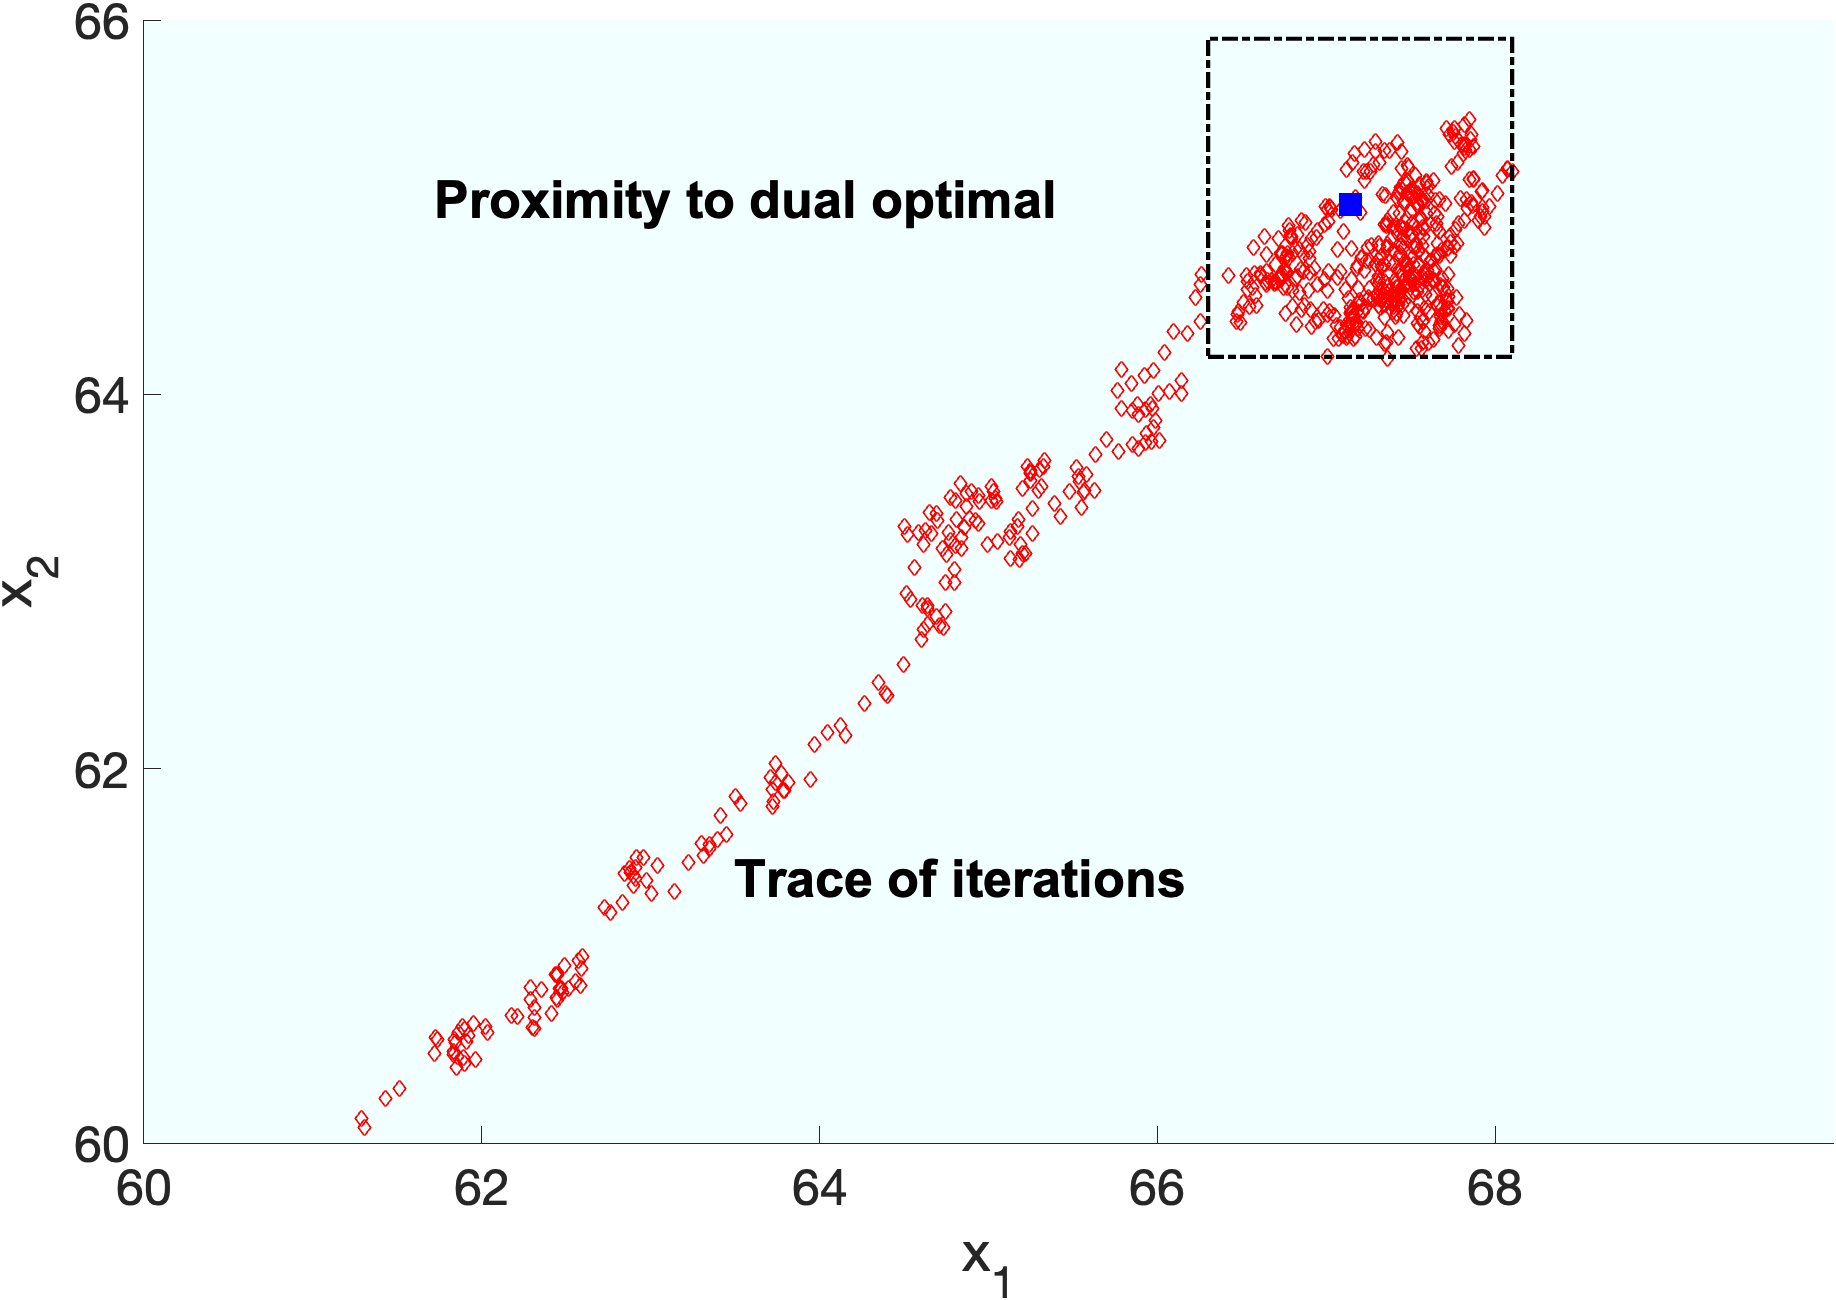
\includegraphics[width=.5\linewidth]{dualcov.png}
    \centering\caption{Dual convergence case}
    \label{fig:dual_cov}
\end{figure}

In this case, the dual price $\bm{p}$ updated by our algorithm can be viewed as a sample of the noised optimal dual price, i.e., $\bm{p}^*$ plus a noise. Similarly, the solution $\tilde{\bm{x}}_{l}$ can also be viewed as the noised optimal solution. Thus, the average solution $\tilde{\bm{x}}^{(K)}$ can reduce the variation of the noise and improves the performance.

From a machine learning perspective, the improvement on the optimality gap can be explained by boosting structure. In some cases, even if the number of duplication times $K$ is small and the dual price $\bm{p}$ marginally moves towards to $\bm{p}^*$, the optimality gap can be reduced significantly, which is also illustrated in Section \ref{sec:exp}. 

According to \cite{friedman2001elements} and \cite{shalev2014understanding}, boosting was originally proposed as a technique for classification problem. Later, there is a line of papers (\cite{frossyniotis2004clustering},\cite{okabe2018clustering}) that extend the boosting technique to solve clustering problems. The essential idea of boosting is to combine a set of weak classifiers to produce a new learner whose performance is significantly better than each weak classifier. To see the structure of boosting in our algorithm, we first construct a cluster problem from \eqref{eqn:sLP}. From the KKT condition \eqref{SOA_dec} and the Assumption \ref{ass:bdd} (c), we know that at most $m$ entries in the optimal solution $\bm{x}^*$ is not 0 or 1. Thus, if $n\gg m$, we can assign a binary index $x^*_j$ for almost every column-coefficient pair $(r_j,\bm{a}_j)$, such that $x^*_j\in\{0,1\}$. With those binary indices, we can view each column-coefficient pair as a sample, each binary solution $\bm{x}\in\{0,1\}^{n}$ as a result of cluster, and each relaxed solution $\tilde{\bm{x}}\in[0,1]^{n}$ as the index score. That is, if its index score $x_j$ is close to 1, the $j$-th sample is deemed to be in the cluster corresponding to 1 with higher probability, which is shown in our algorithm that $\bm{x}$ is a binary solution constructed by rounding the index score vector $\bm{x}^{(K)}$. Thus, in this case, solving the \eqref{eqn:sLP} is equivalent to finding the index scores $\bm{x}$ for all samples to minimize the following function

 \begin{align*}
    L_{\text{OPT}}(\bm{x})
    =
    \left\{
    \begin{matrix}
        &\sum\limits_{j=1}^{n}r_j(x_j^*-x_j), & \text{ if $\bm{A}\bm{x}\leq\bm{b},\ \bm{0}\leq\bm{x}\leq\bm{1}$,}\\
        &\infty, & \text{otherwise,}    
    \end{matrix}
    \right.   
 \end{align*}
 since this function is a equivalent form of \eqref{eqn:LP}. Thus, we can set the loss function for this clustering problem as 
 \begin{align*}
    L(\bm{x})
    =
    \left\{
    \begin{matrix}
        &\sum\limits_{j=1}^{n}r_jx_j, & \text{ if $\bm{A}\bm{x}\leq\bm{b},\ \bm{0}\leq\bm{x}\leq\bm{1}$}\\
        &\infty, & \text{otherwise,}    
    \end{matrix}
    \right.   
 \end{align*}
 which does not depend on the unknown true index $\bm{x}^*$ since $\text{OPT}=\sum\limits_{j=1}^{n}r_jx_j^*$ is a fixed value for \eqref{eqn:LP}. Moreover, if we view $\bm{x}_l$ as a "weak" clustering learner of this cluster problem, the average solution is one combination of weak learners, which is one essential idea of the boosting method as in \cite{friedman2001elements}. 

\begin{algorithm}[ht!]
\caption{Boosting Simple Algorithm}
\label{alg:BSA}
\begin{algorithmic}[1]
\State Input: $\bm{d}=\bm{b}/n$, $K$, $\gamma=1/\sqrt{Kn}$, $M=\sum\limits_{j=1}^{n}M_j$
\State Initialize $\bm{p} = \bm{0}$, $\left(\tilde{{x}}^{(K)}_1,...,\tilde{{x}}^{(K)}_n\right)=\bm{0}$
\For {$l=1,...,K$}
    \State Generate random permutation $\sigma_l=(s_1,...,s_M)$
    \For {$t=s_1,...,s_M$}
        \State Set 
            $$\tilde{x}_{l,t} = \begin{cases}
            1,& r_{t} >\bm{a}_{t}^\top \bm{p} \\
            0,& r_{t} \le \bm{a}_{t}^\top \bm{p} 
            \end{cases}$$
            \State Compute
            \begin{align*}
                \bm{p} & = \bm{p} + \gamma \left(\bm{a}_{t}\tilde{x}_{l,t} - \bm{d}\right) \\
                \bm{p} & = \bm{p} \vee \bm{0}
            \end{align*}
        \State Compute $j'=\min\left\{j: t<\sum\limits_{j_0=1}^{j}M_{j_0}\right\}$
        \State Set $\tilde{{x}}^{(K)}_{j'}=\tilde{{x}}^{(K)}_{j'}+\frac{1}{K}\tilde{x}_{l,t}$
    \EndFor
\EndFor
\For {$t=1,...,n$}
    \State $x_t = [\tilde{{x}}^{(K)}_{t}]+Bernoulli(\tilde{{x}}^{(K)}_{t}-[\tilde{{x}}^{(K)}_{t}])$
\EndFor
\State Output: the binary solution $\bm{x} = (x_1,...,x_n)$ 
\State ~~ ~~ ~~ ~~ the fractional solution $\tilde{\bm{x}}^{(K)}= (\tilde{x}_1^{(K)},...,\tilde{x}_n^{(K)})$
\end{algorithmic}
\end{algorithm}

Now, we solve the \eqref{eqn:LP} by a generalization of Algorithm \ref{alg:bBSA}. To simplify our discussion, we assume $M_j\in\mathbb{N}$ for all $j=1,...,n$. This will not lose the generality because we can always scale the linear program and focus on an equivalent LP as following,
\begin{align*}
    \max \ \ & \sum\limits_{j=1}^{n}\left(\frac{M_j}{[M_j]+1}r_j\right)x_{j}   \\
    \text{s.t. }\ & \sum\limits_{j=1}^{n}\left(\frac{M_j}{[M_j]+1}\bm{a}_j\right)x_{j} \le \bm{b} \nonumber  \\ 
    & x_{j} \in [0,[M_j]+1], \text{ for all } j=1,...,n\nonumber,
\end{align*}
where $[\cdot]$ is the floor function, and the new LP still satisfies Assumption \ref{ass:bdd}. 
In this case, solving the \eqref{eqn:LP} is equivalent to solving the extended LP \eqref{eqn:extLP}.
\begin{align}
   \tag{extLP} \max \ \ & \sum\limits_{j=1}^{n}r_j\left(\sum\limits_{l=1}^{M_j}x_{j,l}\right) \label{eqn:extLP}  \\
    \text{s.t. }\ & \sum\limits_{j=1}^{n}\bm{a}_j\left(\sum\limits_{l=1}^{M_j}x_{j,l}\right) \le \bm{b} \nonumber  \\ 
    & x_{j,l} \in [0,1], \text{ for all } j=1,...,n \text{ and } l=1,...,M_j  \nonumber,
\end{align}
We can find an approximate solution $\{\tilde{x}_{j,l},l=1,...,M_j\}_{j=1}^{n}$ to the \eqref{eqn:extLP}. Then, let $\tilde{x}_j^{(K)}=\sum\limits_{l=1}^{M_j}\tilde{x}_{j,l}$ and 
$$
    x_j^{(K)} = [\tilde{x}_j^{(K)}]+Bernoulli(\tilde{x}_j^{(K)}-[x_j^{(K)}]),
$$
for all $j=1,...,n$. for all $j=1,...,n$. We find a fractional solution $\tilde{x}_j^{(K)}$ and an integer solution $x_j^{(K)}$ of \eqref{eqn:LP}. Algorithm \ref{alg:BSA} summarizes the above discussion.



\subsection{Optimality Gap Analysis}
\label{sec:optgap}
In this section, we present the bounds of optimality gap and constraint violation of the solution obtained by the Boosting Simple Algorithm (Algorithm \ref{alg:BSA}), and the optimality gap of one feasible version of that solution. With Assumption \ref{ass:bdd}, we show that the optimality gaps of both Algorithm \ref{alg:BSA} and Algorithm \ref{alg:bBSA} decrease in the order of $\frac{1}{\sqrt{K}}$ as discussed in Section \ref{sec:Alg}. The proof mainly follows the ideas in \cite{li2020simple}, \cite{balseiro2020dual} and \cite{balseiro2020best}. We leave the proof in the appendix.

\begin{theorem}
The regret and expected constraint violation of the fractional solution $\tilde{\bm{x}}$ obtained from Algorithm \ref{alg:bSOA} satisfy
$$\Delta(\tilde{\bm{x}}) \le O\left(\frac{\sqrt{n}\log n}{\underline{b}\sqrt{K}}  +\frac{m\log nK}{K}\right),$$
$$v(\tilde{\bm{x}}) \le O\left(\sqrt{\frac{m^3n}{\underline{b}^2K}}\right),$$
for all $m, n \in \mathbb{N}^+$.
\label{thm_BSA_cv}
\end{theorem}

To transfer the solution $\tilde{\bm{x}}$ to a feasible solution, we can check the feasibility at each step and terminate the algorithm if one constraint is violated. Denote this feasible fractional solution found by Algorithm \ref{alg:bSOA} as $\bm{x}_{\text{feasible}}$. It satisfies the following theorem. 

\begin{theorem}
The optimality gap of the feasible solution $\bm{x}_{\text{\rm{feasible}}}$ satisfies
$$\Delta({\bm{x}}) \le O\left(\frac{\sqrt{n}\log n}{\underline{b}^2\sqrt{K}}  +\frac{m\log nK}{K}\right),$$
for all $m, n \in \mathbb{N}^+$.
\label{thm_BSA}
\end{theorem}


\subsection{Variants of Binary Boosting Simple Algorithm}
\label{sec:gen}
In this section, we introduce two variants of Algorithm \ref{alg:bBSA}. Recall the discussion in Section \ref{sec:soa} and \ref{sec:boost}, the boosting algorithm combines the ``boosting'' structure and Algorithm \ref{alg:SOA}, and the main idea of Algorithm \ref{alg:SOA} is to apply Projected Stochastic Gradient Descent on the optimization problem \eqref{SA}. To find more variants, one idea is to keep the whole framework same and apply other gradient descent methods. Specifically, we apply Online Mirror Descent and Mini Batch Gradient Descent to the framework. Moreover, in Section \ref{sec:gen}, we compares the numerical performance of those three boosting algorithms. 

First, we introduce Algorithm \ref{alg:bBMD} enlightened by \cite{balseiro2020dual}. This algorithm applies Online Mirror Descent instead of Stochastic Gradient Descent and, thus, have more flexibility to adapt the geometry of the objective function, which will be discussed later. Besides Algorithm \ref{alg:SOA} proposed by \cite{li2020simple}, \cite{balseiro2020dual} and \cite{balseiro2020best} introduce Dual Mirror Descent Algorithm to solve Online LP in linear time concurrently. The main idea of their algorithm is to apply Online Mirror Descent on the problem \eqref{SA}. To introduce the algorithm, we first briefly recall the Online Mirror Descent method (\cite{hazan2019introduction}, \cite{bubeck2011introduction}) when solving the problem \eqref{SA}. When applying Stochastic Gradient Descent, equivalently, we update the approximated solution as the formula below at each iteration to solve \eqref{SA},
\begin{align}
\label{upt:sgd}
    \bm{p}_{t+1} 
    =
    \arg\min\limits_{\bm{p}\in\mathbb{R}^{m}_{+}} \left\{
        \left(\bm{d}-\bm{a}_jI(r_j>\bm{a}_j^{\top}\bm{p}_t)\right)^{\top}\left(\bm{p}-\bm{p}_t\right)
        +
        \frac{n}{2}\|\bm{p}-\bm{p}_{t}\|_2^2
    \right\}.
\end{align}
The first part in the RHS of \eqref{upt:sgd} can be viewed as a first order approximation of the value $f_n(\bm{p})-f_n(\bm{p}_t)$. Specifically, since
\begin{align*}
    f_n(\bm{p})-f_n(\bm{p}_t)
    =
    \left(\left.\frac{\partial f_n(\bm{p})}{\partial \bm{p}}\right\vert_{\bm{p}=\bm{p}_t}\right)^{\top}\left(\bm{p}-\bm{p}_t\right)+o(\|\bm{p}-\bm{p}_t\|_2),
\end{align*}
we can find the first term in \eqref{upt:sgd} by using $\bm{d}-\bm{a}_jI(r_j>\bm{a}_j^{\top}\bm{p}_t)$ to estimate $\frac{\partial f_n(\bm{p})}{\partial \bm{p}}|_{\bm{p}=\bm{p}_t}$. The second part in the RHS of  \eqref{upt:sgd} can be viewed as penalty since the first order approximation has large error when $\bm{p}$ is far from $\bm{p}_t$. Thus, compared with $\bm{p}_t$, the updated dual price $\bm{p}_{t+1}$ reduces function value by roughly $\left(\left.\frac{\partial f_n(\bm{p})}{\partial \bm{p}}\right\vert_{\bm{p}=\bm{p}_t}\right)^{\top}\left(\bm{p}_{t+1}-\bm{p}_t\right)$. However, the approximation error depends on the local curvature of the target function and the two-norm might not be the best penalty for it. Thus, to adapt this local geometry, Online Mirror Descent replaces the two-norm penalty term in \eqref{upt:sgd} with Bregman divergence $V_h$, i.e.
\begin{align}
\label{upt:md}
    \bm{p}_{t+1} 
    =
    \arg\min\limits_{\bm{p}\in\mathbb{R}^{m}_{+}} \left\{
        \left(\bm{d}-\bm{a}_jI(r_j>\bm{a}_j^{\top}\bm{p}_t)\right)^{\top}\left(\bm{p}-\bm{p}_t\right)
        +
        \frac{n}{2}V_h(\bm{p},\bm{p}_t)
    \right\},
\end{align}
where the reference function $h$ is an arbitrary strictly-convex function and
\begin{align*}
    V_h(\bm{p},\bm{p}')
    =
    h(\bm{p})-h(\bm{p}')-(\bm{p}-\bm{p}')\nabla h(\bm{p'}).
\end{align*}
Then, applying the same boosting idea in Section \ref{sec:boost}, we have Algorithm \ref{alg:bBMD}, where $\bm{p}_0$ is the initial vector. When we choose $h(\bm{p})=\frac{1}{2}\|\bm{p}\|_2^2$ and $\bm{p}_0=\bm{0}$, the Algorithm \ref{alg:bBMD} is exact same as Algorithm \ref{alg:bBSA}. In Section \ref{sec:exp}, we will select the function $h$ to be the negative entropy function. In that case, if we still choose $\bm{p}_0=\bm{0}$, we will see that at all iterations, the dual price will always be the zero vector, which cannot provide good solution. Additionally, we can also extend it to solve \eqref{eqn:LP} by apply same process in Section \ref{sec:boost}. For the optimality gap, we can also apply the similar method in Theorem \ref{thm_BSA} and \ref{thm_BSA_cv} to find the similar result.

\begin{algorithm}[ht!]
\caption{Binary Boosting Mirror Descent Algorithm}
\label{alg:bBMD}
\begin{algorithmic}[1]
\State Input: $\bm{d}=\bm{b}/n$, $K$, $\gamma=1/\sqrt{Kn}$
\State Initialize $\bm{p} = \bm{p}_0$, $(\tilde{{x}}^{(K)}_1,...,\tilde{{x}}^{(K)}_n)=\bm{0}$
\For {$l=1,...,K$}
    \State Generate random permutation $\sigma_l=(s_1,...,s_n)$
    \For {$t=s_1,...,s_n$}
        \State Set 
            $$\tilde{x}_{l,t} = \begin{cases}
            1,& r_{t} >\bm{a}_{t}^\top \bm{p}_t \\
            0,& r_{t} \le \bm{a}_{t}^\top \bm{p}_t
            \end{cases}$$
            \State Compute
            \begin{align*}
                \bm{p}_{t+1} & = \arg\min\limits_{\bm{p}\in\mathbb{R}^{m}_{+}} \left\{
                        \left(\bm{d}-\bm{a}_jI(r_j>\bm{a}_j^{\top}\bm{p}_t)\right)^{\top}\left(\bm{p}-\bm{p}_t\right)
                        +
                        nV_h(\bm{p},\bm{p}_t)
                    \right\}
            \end{align*}
            \State Set $\tilde{{x}}^{(K)}_t=\tilde{{x}}^{(K)}_t+\frac{1}{K}\tilde{{x}}_{l,t}$
    \EndFor
\EndFor
\For {$t=1,...,n$}
    \State $x_t = Ber(\tilde{x}_t^{(K)})$
\EndFor
\State Output: the binary solution $\bm{x} = (x_1,...,x_n)$ 
\State ~~ ~~ ~~ ~~ the fractional solution $\tilde{\bm{x}}^{(K)}= (\tilde{x}_1^{(K)},...,\tilde{x}_n^{(K)})$
\end{algorithmic}
\end{algorithm}

Secondly, we propose Algorithm \ref{alg:bBMB} with Mini Batch Gradient Descent. Mini Batch Gradient Descent (\cite{bottou2010large}) is also one important part of gradient descent methods. Compared with Stochastic Gradient Descent, Mini Batch Descent collect several samples at each iteration to update the solution, which is more stable and has low variance at each step. To be specific, for Stochastic Gradient Descent, we iteratively update dual price with single sample by
$$
    \bm{p}_{t+1}
    =
    \bm{p}_t
    -
    \frac{1}{n}(\bm{d}-\bm{a}_t I(r_t>\bm{a}_t^{\top}\bm{p}_t)).
$$

\begin{algorithm}[ht!]
\caption{Binary Boosting Mini Batch Algorithm}
\label{alg:bBMB}
\begin{algorithmic}[1]
\State Input: $\bm{d}=\bm{b}/n$, $K$, $\gamma=1/\sqrt{Kn}$
\State Input: batch size $s$
\State Initialize $\bm{p} = \bm{0}$, $(\tilde{{x}}^{(K)}_1,...,\tilde{{x}}^{(K)}_n)=\bm{0}$
\For {$l=1,...,K$}
    \State Generate random permutation $\sigma_l=(s_1,...,s_n)$
    \For {$t=1,2,...,n$}
        \State Set 
            $$\tilde{x}_{l,t} = \begin{cases}
            1,& r_{t} >\bm{a}_{t}^\top \bm{p}_t \\
            0,& r_{t} \le \bm{a}_{t}^\top \bm{p}_t
            \end{cases}$$
            \If {$t$ is dividable by $s$}
            \State Compute
            \begin{align*}
                \bm{p}_{t+1} & = \bm{p}_t
                -
                 \frac{1}{ns}\sum\limits_{j'=0}^{s-1}(\bm{d}-\bm{a}_{t-j'} I(r_{t-j'}>\bm{a}_{t-j'}^{\top}\bm{p}_t))
            \end{align*}
            \Else
            \State Set $\bm{p}_{t+1}  = \bm{p}_t$
            \EndIf
            \State Set $\tilde{{x}}^{(K)}_t=\tilde{{x}}^{(K)}_t+\frac{1}{K}\tilde{{x}}_{l,t}$
    \EndFor
\EndFor
\For {$t=1,...,n$}
    \State $x_t = Ber(\tilde{x}_t^{(K)})$
\EndFor
\State Output: the binary solution $\bm{x} = (x_1,...,x_n)$ 
\State ~~ ~~ ~~ ~~ the fractional solution $\tilde{\bm{x}}^{(K)}= (\tilde{x}_1^{(K)},...,\tilde{x}_n^{(K)})$
\end{algorithmic}
\end{algorithm}

Alternatively, for Mini Batch Descent, once the algorithm collect $s$ samples at an iteration, it updates the dual price by
$$
    \bm{p}_{t+s}
    =
    \bm{p}_t
    -
    \frac{1}{ns}\sum\limits_{j'=0}^{s-1}(\bm{d}-\bm{a}_{t+j'} I(r_{t+j'}>\bm{a}_{t+j'}^{\top}\bm{p}_t)),
$$
where $s$ is a given integer.
This basically describes Algorithm \ref{alg:bBMB}, another variant of the boosting algorithm.

\subsection{Application in Column Generation}
\label{sec:cg}
In this section, the boosting algorithms are applied as the initialization of Column Generation methods and the Sifting Procedures to accelerate the process of solving large-scale LPs. Moreover, in this part, we no longer require the resources vector to be positive. First, let us briefly revisit the concept of Column Generation (\cite{lubbecke2005selected})and Sifting(\cite{bixby1992very}). Column Generation method is first proposed by \cite{ford1958suggested}. Assuming that most variables in an large-scale LP would be non-basic and take zero values in the optimal solution. Column Generation methods only consider variables likely to be in the basis instead of all variables. Specifically, In the Column Generation procedure, we call the LP below \eqref{eqn:MLP} as the Master Problem (MP),
\begin{align*}
   \tag{MP} \max \ \ & \sum\limits_{j=1}^{n}r_j x_j \label{eqn:MLP}  \\
    \text{s.t. }\ & \sum\limits_{j=1}^{n}\bm{a}_j x_j \le \bm{b} \nonumber  \\ 
    & x_j \ge 0, \ \ j=1,...,n \nonumber,
\end{align*}
where $\bm{a}_i \in \R^{m}$ for all $i=1,...,n$ and $\bm{b} = (b_1,...,b_m)^{\top} \in \R^m$. Instead of solving the Master Problem directly, we only solve problems restricted to part of variables in the Master Problem,
\begin{align*}
   \tag{RMP} \max \ \ & \sum\limits_{j\in J}r_j x_j \label{eqn:RLP}  \\
    \text{s.t. }\ & \sum\limits_{j\in J}\bm{a}_j x_j \le \bm{b} \nonumber  \\ 
    & x_j \ge 0, \ \ j\in J \nonumber,
\end{align*}
where the index set $J$ is a subset of $\{1,...,n\}$. We call this subproblem the Restricted Master Problem (RMP). Let $\bm{x}_{\text{RMP}}^*$, $\bm{p}_{\text{RMP}}^*$ be the optimal primal and dual price corresponding to the subproblem, respectively, and $c^*$ be the minimal reduced cost with respect to $\bm{p}_{\text{RMP}}^*$, namely, 
$$
   c^* = \min_{j=1,..,n}\{ \bm{a}_j^{\top}\bm{p}_{\text{RMP}}^* - r_j \}.
$$
After finding the RMP, the Column Generation oracle returns whether $c^*$ is non-negative. If $c^*\geq0$, all reduced costs are non-negative and, thus, the optimal solution of RMP \eqref{eqn:RLP} is also an optimal solution of MP \eqref{eqn:MLP}. We then finish the procedure and can solve RMP to obtain the optimal solution of MP. Otherwise, the oracle will also generate one or several columns whose corresponding reduced costs are strictly negative. We then add them to the index set $J$, and repeat the procedure until $c^*\geq0$. Sifting Procedure is one important Column Generation method. Specifically, during the procedure, Sifting method computes reduced costs for all columns, and select one or several columns with smallest reduced costs to put into the index set $J$. Although computing all reduced costs is computationally expensive, due to the development of current computing power, Sifting is often a powerful tool to solve LP and it is widely implemented in most state-of-the art LP solvers, such as COPT, Gurobi and CPLEX. 

Although it is useful, Column Generation Methods still suffers from several issues (\cite{vanderbeck2005implementing}), such as the heading-in effect, the tailing off effect, and the bang-bang effect.  Specifically, the heading-in effect is the phenomenon that due to insufficient prior knowledge, the index set $J$ of the initial RMP has small overlap with the set of indices of non-zero variables in the optimal solution so that the algorithm spends long time to starting to increase the objective value at the beginning. The tailing off effect is the phenomenon that the convergence of the duality gap is very slow, where the duality gap is the difference between the primal optimal objective value of the RMP and the dual objective value of original problem with respect to the dual price $\bm{p}_{RMP}^*$. The bang-bang effect is the case that the dual solutions obtained by RMPs jump form one extreme point to another. In this section, we apply our boosting algorithm to moderate heading-in effect and the bang-bang effect to accelerate Column Generation Procedure.

First, to moderate the heading-in effect, the boosting algorithms can be applied to better identify non-zero variables in the true optimal solution to formulate the initial RMP. Intuitively, given that our algorithm can find good approximate solution of LPs, it is reasonable to believe that the variables have large value in the solution obtained by our boosting algorithms tend to be more likely to have contribution in the true optimal solution. Thus, we can directly initialize the Column Generation procedure with with variables with large values in the solution obtained by the boosting algorithms. Specifically, we can set up any thresholds $\epsilon$ and the the duplication size $K$ in the beginning, apply our boosting algorithm to obtain a fraction solution $\tilde{\bm{x}}^{(K)}$, and set 
$$
    J=\left\{j\in\{1,...,n\}: \tilde{x}_j^{(K)}>\epsilon\right\}
$$
as the index set of the initial RMP. 

Moreover, to moderate the bang-bang effect, we combine the dual price with the dual stabilization technique to accelerate Sifting procedure. The stabilization technique is widely used in Column Generation (\cite{du1999stabilized}, \cite{amor2004stabilization}, \cite{lubbecke2005selected}, and \cite{2011Chebyshev}). This technique has two main ideas: finding a good stabilization center of the dual price and searching for new dual prices around the center. According to \cite{lubbecke2010column}, a good stabilization center is believed to be close to true dual optimal solution or at least an interior point of dual space. Recall that Algorithm \ref{alg:BSA} carries out stochastic descent in dual space and, thus, the dual price obtained by Algorithm \ref{alg:BSA} is probably a high-quality dual solution. Hence we may choose it as the stabilization center and denote this dual price by $\bm{p}_{\text{Online}}$. Once we have this center, at each step during the Sifting, we compute reduced cost by
$$
    \hat{\bm{p}} = \alpha \bm{p}^*_{\text{RMP}} + (1-\alpha) \bm{p}_{\text{Online}}
$$
instead of $\bm{p}^*_{\text{RMP}}$, where $\alpha>0$ is a parameter chosen by the algorithm designer. In this case, once this dual price is close to dual optimal solution $\bm{p}^*$, we can expect good stabilization effect and acceleration. Then, we can combine the initialization part and this stabilization part together to have a boosting algorithm based Column Generation method.






\section{Numerical Experiments}
\label{sec:exp}
In this section, we present some numerical results for our proposed algorithms. Section \ref{sec:solver} illustrates the performance of boosting algorithms as direct LP solvers. Section \ref{sec:cg} applies the boosting algorithms as the initialization and a  of Column Generation methods for solving large scale LPs.


\subsection{Approximate Solver}
\label{sec:solver}
In this section, we apply boosting algorithms as approximate algorithms to solve LPs/integer LPs. To this end, we only compare the performance of feasible solutions in this section.  

The first experiment compares the performance of the feasible fractional solution obtained by Algorithm \ref{alg:SOA}, Algorithm \ref{alg:bBSA} and Gurobi in terms of time (millisecond) and competitiveness ratio, where the competitiveness ratios are the ratio between the objective obtained by the given algorithms against the relaxed LP's optimal objective value solved by Gurobi. Here, Simple Online Algorithm \ref{alg:SOA} is a special case for the Algorithm \ref{alg:bBSA} when $K=1$. We test our algorithms on the linear relaxation of some Multi-knapsack benchmark problems \citep{chu1998genetic} with different duplication sizes $K=10,50,10^3$ and different orders of resources vectors $\bm{b}$, namely, $O(n)$, $O(n^{1/2})$ and $O(n^{1/3})$ in this experiment. 
According to \cite{chu1998genetic}, this binary knapsack problems are dense and the resources vectors $\bm{b}$ they generate are in the order of $n$. In our experiments, we modify the order of resources vector from $O(n)$ to $O(n^\alpha)$ by multiplying a factor $n^{\alpha-1}$ to their resources vectors for any $\alpha\in(0,1]$. For each choice of $m$ and $n$, we run $100$ simulation trials and present the average time and ratio. 
The results are shown in Table \ref{tab:sol_1}, \ref{tab:sol_1/2} and \ref{tab:sol_1/3}. From the tables, we observe that the ratio increases when the duplication size increases from $10$ to $10^3$ for all cases. Further, when $K=10$ or $50$, the ratio is roughly no less than than $90\%$ or $95\%$ respectively for different orders of resources vector and different sizes of problems, which is $10\%$ or even $40\%$ better than Algorithm \ref{alg:SOA}. We can conclude that the boosting algorithm can better utilize the data than Algorithm \ref{alg:SOA} and find a better solution even though the resources vector is sublinear. This phenomena is consistent with our theorem \ref{thm_BSA}. Moreover, our algorithm is also time-efficient for large problems. As shown in the tables, the running time of Algorithm \ref{alg:BSA} with $K=10$ is from one sixth to one thirtieth compared with Gurobi when $m=128,\ n=10^5$, although we did not apply any accelerating methods for vector computing, such as parallely computing vector multiplications.

\begin{table}[ht!]
    \centering
    \small
    \begin{tabular}{cc|c|c|c|c|c}
    \toprule
         && Gurobi  & Alg. \ref{alg:SOA} & Alg. \ref{alg:BSA} ($K=10$) & Alg. \ref{alg:BSA} ($K=50$) & Alg. \ref{alg:BSA}  ($K=10^3$) \\
         \midrule
   \multirow{2}{*}{\scriptsize $m=5, n=10^2$}  & time & 1.00 & 0.02 & 0.08 & 0.35 & 6.72 \\
   & Cmpt. Ratio &100.0\% & 80.2\% & 93.3 \% & 96.8\% & 99.5\%  \\
\midrule
  \multirow{2}{*}{\scriptsize $m=8, n=10^3$} &  time  & 1.99 & 0.22 & 1.20 & 5.90 & 93.17  \\ 
   &Cmpt. Ratio & 100.0\% & 86.4\% & 95.4\% & 98.1\% & 99.7\%   \\
\midrule
    \multirow{2}{*}{\scriptsize $m=32, n=4\times10^3$} &  time   &  49.8  & 1.29 & 18.11 & 79.50 & 1250  \\ 
  & Cmpt. Ratio & 100.0\% & 74.2\% & 89.1\% & 95.0\% & 99.2\% \\
\midrule
    \multirow{2}{*}{\scriptsize $m=64, n=10^4$} &  time   &  285.7  & 6.53 & 88.79 & 391.53 & 6420 \\ 
  & Cmpt. Ratio & 100\% & 70.5\% & 86.1\% & 93.3\% & 98.7\% \\ 
\midrule
    \multirow{2}{*}{\scriptsize $m=128, n=10^5$} &  time   &  12600  & 150.52 & 1980 & 8610 & 143000  \\ 
  & Cmpt. Ratio & 100\% & 76.4\% & 90.4\% &  95.6\% & 99.1\% \\  
   \bottomrule
    \end{tabular}
        \caption{Linear Relaxation of Multi-knapsack Benchmark Problem with $\bm{b}\sim O(n)$}
    \label{tab:sol_1}
\end{table}

\begin{table}[ht!]
    \centering
    \small
    \begin{tabular}{cc|c|c|c|c|c}
    \toprule
         && Gurobi  & Alg. \ref{alg:SOA} & Alg. \ref{alg:BSA} ($K=10$) & Alg. \ref{alg:BSA} ($K=50$) & Alg. \ref{alg:BSA}  ($K=10^3$) \\
         \midrule
   \multirow{2}{*}{\scriptsize $m=5, n=10^2$}  & time & 1.00 & 0.02 & 0.08 & 0.35 & 6.72 \\
   & Cmpt. Ratio &100.0\% & 64.4\% & 90.3\% & 96.1\% & 99.5\%  \\
\midrule
  \multirow{2}{*}{\scriptsize $m=8, n=10^3$} &  time  & 3.10 & 0.22  & 1.20 & 5.90 & 93.17  \\ 
   &Cmpt. Ratio & 100.0\% & 80.2\% & 95.0\% & 98.1\% & 99.7\%   \\
\midrule
    \multirow{2}{*}{\scriptsize $m=32, n=4\times10^3$} &  time   &  75.4  & 1.29 & 18.11 & 79.50 & 1250  \\ 
  & Cmpt. Ratio & 100.0\% & 80.1\% & 93.2\% & 96.8\% & 99.2\% \\
\midrule
    \multirow{2}{*}{\scriptsize $m=64, n=10^4$} &  time   &  303.2  & 6.53 & 88.79 & 391.53 & 6420 \\ 
  & Cmpt. Ratio & 100\% & 81.0\% & 92.3\% & 96.1\% & 98.7\% \\ 
\midrule
    \multirow{2}{*}{\scriptsize $m=128, n=10^5$} &  time   &  12600  & 150.52 & 1980 & 8610 & 143000  \\ 
  & Cmpt. Ratio & 100\% & 87.6\% & 94.8\% & 97.2\% & 99.1\% \\  
   \bottomrule
    \end{tabular}
        \caption{Linear Relaxation of Multi-knapsack Benchmark Problem with $\bm{b}\sim O(n^{1/2})$}
    \label{tab:sol_1/2}
\end{table}

\begin{table}[ht!]
    \centering
    \small
    \begin{tabular}{cc|c|c|c|c|c}
    \toprule
         && Gurobi  & Alg. \ref{alg:SOA} & Alg. \ref{alg:BSA} ($K=10$) & Alg. \ref{alg:BSA} ($K=50$) & Alg. \ref{alg:BSA}  ($K=10^3$) \\
         \midrule
   \multirow{2}{*}{\scriptsize $m=5, n=10^2$}  & time & 0.51 & 0.02 & 0.08 & 0.35 & 6.72 \\
   & Cmpt. Ratio &100.0\% & 41.3\% & 85.8\% &  96.3\% & 99.3\%  \\
\midrule
  \multirow{2}{*}{\scriptsize $m=8, n=10^3$} &  time  & 3.4 & 0.22  & 1.20 & 5.90 & 93.17  \\ 
   &Cmpt. Ratio & 100.0\% & 58.6\% & 92.2\% & 96.8\% & 99.2\%   \\
\midrule
    \multirow{2}{*}{\scriptsize $m=32, n=4\times10^3$} &  time   &  76.1  & 1.29 & 18.11 & 79.50 & 1250  \\ 
  & Cmpt. Ratio & 100.0\% & 65.1\% & 91.2\% &  96.7\% & 99.5\% \\
\midrule
    \multirow{2}{*}{\scriptsize $m=64, n=10^4$} &  time   &  355.1  & 6.53  & 88.79 & 391.53 & 6420 \\ 
  & Cmpt. Ratio & 100\% & 67.1\% &  91.5\% & 97.4\% & 99.5\% \\ 
\midrule
    \multirow{2}{*}{\scriptsize $m=128, n=10^5$} &  time   &  70100  & 150.52 & 1980&  8610 & 143000  \\ 
  & Cmpt. Ratio & 100\% & 78.7\% & 94.7\% & 98.0\% & 99.6\% \\  
   \bottomrule
    \end{tabular}
        \caption{Linear Relaxation of Multi-knapsack Benchmark Problem with $\bm{b}\sim O(n^{1/3})$}
    \label{tab:sol_1/3}
\end{table}


The second experiment compares the performance of Algorithm \ref{alg:BSA} with Gurobi when solving large-scale sparse LPs and also present the time (millisecond) and the competitive ratio. Again, the competitiveness ratios are the ratio between the objective obtained by given algorithms against the relaxed LP's optimal objective value solved by Gurobi. To generate the sparse problem, we first generated a dense problem according to \cite{chu1998genetic} and, then, randomly choose $0.01mn$ non-zero entry in the dense resources consumption matrix $\bm{A}$. Then, we test our algorithms on the data generated similarly as the benchmark data with different duplication sizes, namely, $K=10,\ 50,\ 10^3$, and order of resources vectors. Also, for each choice of $m$ and $n$, we run $100$ simulation trials and present the average time and ratio in Table \ref{tab:solsp_1}, \ref{tab:solsp_1/2} and \ref{tab:solsp_1/3}. As shown in those tables, when $K=10$, the computational time of our algorithm is around $2\times 10^3$ milliseconds, which is slightly better than Gurobi. In the case that the resources vector is in the order of $n$, the running time of our algorithm can be one fourth of Gurobi. Moreover, when $K=10$, the ratio of our algorithm is already better than $95\%$ in average, which approximately is the optimal solution. Thus, our algorithm could also be competitive with Gurobi even in some sparse problems.



\begin{table}[ht!]
    \centering
    \small
    \begin{tabular}{cc|c|c|c|c}
    \toprule
         && Gurobi  & Alg. \ref{alg:BSA} ($K=10$) & Alg. \ref{alg:BSA} ($K=50$) & Alg. \ref{alg:BSA}  ($K=10^3$) \\
         \midrule
   \multirow{2}{*}{\scriptsize $m=64, n=10^4$}  & time & 12.2 & 3.36 & 12.13 & 250.78 \\
   & Cmpt. Ratio &100.0\%  & 99.0\% & 93.3\% & 99.9\%  \\
\midrule
  \multirow{2}{*}{\scriptsize $m=128, n=10^5$} &  time  & 474 & 55.04 &  246.07  & 3800  \\ 
   &Cmpt. Ratio & 100.0\% & 99.5\% & 95.6\% & 99.9\%   \\
\midrule
    \multirow{2}{*}{\scriptsize $m=1024, n=10^6$} &  time   &  7980  & 2020 & 8320 & 15500  \\ 
  & Cmpt. Ratio & 100.0\% &  96.5\% & 95.7\% & 99.5\% \\
   \bottomrule
    \end{tabular}
        \caption{Sparse Linear Relaxation of Multi-knapsack Benchmark Problem with $\bm{b}\sim O(n)$}
    \label{tab:solsp_1}
\end{table}

\begin{table}[ht!]
    \centering
    \small
    \begin{tabular}{cc|c|c|c|c}
    \toprule
         && Gurobi  & Alg. \ref{alg:BSA} ($K=10$) & Alg. \ref{alg:BSA} ($K=50$) & Alg. \ref{alg:BSA}  ($K=10^3$) \\
         \midrule
   \multirow{2}{*}{\scriptsize $m=64, n=10^4$}  & time & 12.2 & 3.36 & 12.13 & 250.78 \\
   & Cmpt. Ratio &100.0\% &  94.8\% & 96.0\% & 94.8\%  \\
\midrule
  \multirow{2}{*}{\scriptsize $m=128, n=10^5$} &  time  & 474.4 & 55.04 &  246.07  & 3800  \\ 
   &Cmpt. Ratio & 100.0\% & 91.2\% & 97.3\% & 91.6\%   \\
\midrule
    \multirow{2}{*}{\scriptsize $m=1024, n=10^6$} &  time   &  3580  & 2020 & 8320 & 15500  \\ 
  & Cmpt. Ratio & 100.0\% & 96.5\% & 98.8\% & 99.4\% \\
   \bottomrule
    \end{tabular}
        \caption{Sparse Linear Relaxation of Multi-knapsack Benchmark Problem with $\bm{b}\sim O(n^{1/2})$}
    \label{tab:solsp_1/2}
\end{table}

\begin{table}[ht!]
    \centering
    \small
    \begin{tabular}{cc|c|c|c|c}
    \toprule
         && Gurobi  & Alg. \ref{alg:BSA} ($K=10$) & Alg. \ref{alg:BSA} ($K=50$) & Alg. \ref{alg:BSA}  ($K=10^3$) \\
         \midrule
   \multirow{2}{*}{\scriptsize $m=64, n=10^4$}  & time & 12.2 & 3.36 & 12.13 & 250.78 \\
   & Cmpt. Ratio &100.0\% & 94.8\% & 97.0\% & 97.4\%  \\
\midrule
  \multirow{2}{*}{\scriptsize $m=128, n=10^5$} &  time  & 130.3 & 55.04 &  246.07  & 3800  \\ 
   &Cmpt. Ratio & 100.0\% & 91.2\% & 97.8\% &  96.7\%   \\
\midrule
    \multirow{2}{*}{\scriptsize $m=1024, n=10^6$} &  time   &  2750  & 2020 & 8320 & 15500  \\ 
  & Cmpt. Ratio & 100.0\% & 99.2\% & 91.3\% & 99.2\% \\
   \bottomrule
    \end{tabular}
        \caption{Sparse Linear Relaxation of Multi-knapsack Benchmark Problem with $\bm{b}\sim O(n^{1/3})$}
    \label{tab:solsp_1/3}
\end{table}


The third experiment compares the performance of Algorithm \ref{alg:BSA}, \ref{alg:bBMD} and \ref{alg:bBMB} on the linear relaxation of knapsack benchmark problem. In this part, we only compares the competitiveness ratio since, theoretically, all of three algorithms share the same computational complexity. As previous experiments, we also test our algorithms with different duplication sizes, namely $K=10$ and $50$. In addition, we set $\bm{p}_0 = \bm{1}/\exp$ and select the reference function $h(\bm{p})$ of the Algorithm \ref{alg:bBMD} to be the negative entropy function
$$
    h(\bm{p})
    =
    \sum\limits_{j=1}^{m}p_i\log p_i,
$$
where $\bm{p}=(p_1,...,p_m)^{\top}\in\mathbb{R}^m$. In this case, the corresponding Bregman divergence coincides with the generalized KL divergence, and dual price updating also only costs constant time at iteration $t$, namely, 
\begin{align}
    \label{eqn:uptkl}
    \bm{p}_{t+1} = \exp\left\{-\gamma(\bm{d}-\bm{a}_{t} x_{t})\right\}\bm{p}_t,    
\end{align}
where the multiplication and the exponential function is computed entry-wisely. Here, we can set $\bm{p}_0$ to be any strictly positive vector theoretically (\cite{balseiro2020best}). Moreover, for Algorithm \ref{alg:bBMB}, we set the batch size be 10. The results are listed in Table \ref{tab:bs10} and \ref{tab:bs50}. First, we observe that all algorithms perform better when the duplication size increase. This improvement along with the duplication size is consistent with our theoretical results. in this experiment, Algorithm \ref{alg:bBMD} can achieve better competitive ratio with lower duplication size than others when the resources vector is relatively large, especially when the vector is in the order of $O(n)$. However, when the order of the resources vector decreases to $1/3$ and the size of $n$ raises to $10^5$, Algorithm \ref{alg:bBMD} has poor performance and can only achieve no more than $40\%$ competitive ratio. One possible reason is that the updating process \eqref{eqn:uptkl} is very slow for Algorithm \ref{alg:bBMD} in this case since the vector $\bm{d}$ is very small. Then, all dual price obtained by this algorithm are close to the initialization price. Thus, if the initial estimation overestimates the dual price, this algorithm is likely to set 0 for all decision variables. This result suggests that one should be careful when choosing the reference function and the initialization for Algorithm \ref{alg:bBMD} based on the data. 

\begin{table}[H]
        \centering
        \small
        \begin{tabular}{c|c|c|c|c}
        \toprule
            $K=10$ & Order of $\bm{b}$  & Alg. \ref{alg:bBSA}& Alg. \ref{alg:bBMD} & Alg. \ref{alg:bBMB} \\
             \midrule
       \multirow{3}{*}{\scriptsize $m=8, n=10^3$}  & $O(n)$ & $95.4\%$ & $99.0\%$  & $99.2\%$\\
        &$O(n^{1/2})$ & 95.0\% & 95.5\% & 85.7\%  \\
        &$O(n^{1/3})$ & 92.1\% & 89.9\% & 54.0\%  \\
    \midrule
       \multirow{3}{*}{\scriptsize $m=64, n=10^4$}  & $O(n)$ & $86.1\%$ & $99.7\%$  & $98.2\%$ \\
        &$O(n^{1/2})$ & 92.3\% & 69.4\% & 96.0\%  \\
        &$O(n^{1/3})$ & 92.1\% & 0.0\% & 84.8\%  \\
    \midrule
       \multirow{3}{*}{\scriptsize $m=128, n=10^5$}  & $O(n)$ & $90.4\%$ & $99.9\%$  & $98.9\%$ \\
        &$O(n^{1/2})$ & 94.8\% & 60.6\% & 97.6\%  \\
        &$O(n^{1/3})$ & 94.7\% & 0.0\% & 89.4\%  \\
       \bottomrule
        \end{tabular}
            \caption{Competitive Ratios of Boosting Algorithms with Duplication Size $K=10$}
        \label{tab:bs10}
\end{table}
\begin{table}[ht!]
        \centering
        \small
        \begin{tabular}{c|c|c|c|c}
        \toprule
            $K=50$ & Order of $\bm{b}$  & Alg. \ref{alg:bBSA}& Alg. \ref{alg:bBMD} & Alg. \ref{alg:bBMB} \\
             \midrule
       \multirow{3}{*}{\scriptsize $m=8, n=10^3$}  & $O(n)$ & $98.1\%$ & $99.6\%$  & $99.7\%$\\
        &$O(n^{1/2})$ & 98.1\% & 98.2\% & 93.3\%  \\
        &$O(n^{1/3})$ & 96.5\% & 96.8\% & 77.1\%  \\
    \midrule
       \multirow{3}{*}{\scriptsize $m=64, n=10^4$}  & $O(n)$ & $93.3\%$ & $99.8\%$  & $99.5\%$ \\
        &$O(n^{1/2})$ & 96.1\% & 86.3\% & 98.1\%  \\
        &$O(n^{1/3})$ & 97.4\% & 37.5\% & 93.1\%  \\
    \midrule
       \multirow{3}{*}{\scriptsize $m=128, n=10^5$}  & $O(n)$ & $95.6\%$ & $99.9\%$  & $99.7\%$ \\
        &$O(n^{1/2})$ & 97.2\% & 82.4\% & 99.1\%  \\
        &$O(n^{1/3})$ & 98.0\% & 0.0\% & 94.5\%  \\
       \bottomrule
        \end{tabular}
            \caption{Competitive Ratios of Boosting Algorithms with Duplication Size $K=50$}
        \label{tab:bs50}
\end{table}

\subsection{Column Generation}
\label{sec:expcg}
In this section, we present performance the application of our boosting algorithm in Column Generation methods as discussed in Section \ref{sec:cg}. We select thirteen benchmark datasets from \textbf{MIPLIB} (\cite{MIPLIB}) and \textbf{Mittelmann Hans' LP Benchmark}. These problems feature $n \gg m$, high sparsity and cover type constraints. 

The first experiment presents the performance of our boosting algorithm for initializing Column Generation. Recall the first part in Section \ref{sec:cg} that to initialize the Column Generation, we can run Algorithm \ref{alg:BSA} or \ref{alg:bBMD} to find an approximate solution $\bm{x}^{(K)}$ and select columns $j$ into the initial index set of RMP if $x_j^{(k)}>\epsilon$, where $\epsilon$ is a threshold chosen by the user. Let $J$ denote the index set of selected columns, $\mathcal{B}^*$ denote the index set of non-zero optimal solutions and $n$ denote the total number of variables. In Table \ref{tab:varidy}, we compare the number of selected columns in the optimal solution $\vert J\cap \mathcal{B}^*\vert$ with the number of non-zero optimal solutions as the accuracy of the selection $\vert\mathcal{B}^*\vert$, and compare the number of selected columns $\vert J\vert$, i.e., the number of variables in the RMP, with the total number of variables $n$ as the size reduction of the original problem. We observe that our algorithm can detect $90$ percents of non-zero variables for first ten data sets and reduce the size of problem by one fifth to one fiftieth. Especially for sixth to tenth problems, our algorithm can find all non-zero variables and reduce the size to at most one fiftieth. This result illustrates that our boosting algorithm might be very useful to accelerate Column Generation and moderate the heading-in effect on some kind of set covering problems.

\begin{table}[ht!]
\label{tab:varidy}
\small
\centering
\begin{tabular}{c|c|c|c}
  \hline
  ID & Dataset & Accuracy & Size Reduction\\
  \hline
  1 & rail507 & 271/301 & 11862/62171\\
  2 & rail516 & 121/138 & 8572/46978\\
  3 & rail582 & 325/347 & 12465/54315\\
  4 & rail2586 & 1536/1672 & 145373/909940\\
  5 & rail4284 & 1951/2042 & 348135/1090526\\
  6 & scpm1 & 2754/2754 & 10352/500000\\
  7 & scpn2 & 3411/3411 & 20860/1000000\\
  8 & scpl4 & 1149/1149 & 5718/200000\\
  9 & scpj4scip & 552/552 & 3635/99947\\
  10 & scpk4 & 930/930 & 4077/100000\\
  11 & s82 & 1992/3020 & 52383/1687859\\
  12 & s100 & 150/487 & 835/364203\\
  13 & s250r100 & 415/747 & 3080/270323\\
  \hline
\end{tabular}
\caption{Basic variable identification}
\end{table}

The second experiment compares the performance of the CPLEX Sifting solver, the CPLEX concurrent solver, the CPLEX dual simplex solver and our boosting algorithm-based Sifting method discussed in the second part in Section \ref{sec:cg}. We use the latest stable build of CPLEX (12.1.0) and briefly explain the behavior of the above solvers.

\begin{itemize}
	\item The CPLEX Sifting solver will use all available threads to run the Sifting (Column Generation) algorithm.
	\item The CPLEX concurrent solver spends most threads on the barrier method and three remaining threads (if available) on  the primal simplex method, dual simplex method and sifting algorithm method mentioned above in parallel. Once one of the above algorithm successfully solves the problem, the solver whole routine finishes.
	\item The CPLEX dual simplex solver utilizes all available threads to run dual simplex method.
	\item Our boosting Sifting Method is implemented in Python using the CPLEX concurrent solver for the RMPs. Specially, we shut down sifting when solving the RMPs and implement some basic heuristics (e.g., dual stabilization) to accelerate our sifting method.  
\end{itemize}

\begin{remark}
All our experiment results related to Sifting are implemented and compared with CPLEX instead of Gurobi since CPLEX provides a more flexible API for us to incorporate our boosting heuristic.
\end{remark}

Here, we use the same data sets as the previous experiment, and show time (second) that listed algorithms take to find the optimal solution in table \ref{tab:sifting}. Also, to demonstrate the robustness of our method, we presolve the problems before running the boosting algorithm.
From the table, we can see that our algorithm is roughly the fastest one in problem 6 to 10 in which all non-zero variables are detected by our boosting algorithm. Moreover, even if our algorithm cannot detect all non-zero optimal variables, our algorithm can still be faster than CPLEX Sifting among problem 12 and 13. This result illustrates that our algorithm has potential to accelerate Column Generation method. Furthermore, in those two experiments, the problems are set cover problems. In other words, the resources vectors can be negative in this case. Thus, the numerical results shows that our algorithm might be useful in solving more general LPs. Also, since our sifting implementation calls CPLEX as a subroutine and spends much time transferring data, we believe that there is still space for improvement if our boosting method can be directly embedded within the solver as a presolving heuristic.

\begin{table}[ht!]
\small
\label{tab:sifting}
\centering
\begin{tabular}{c|c|c|c|c|c|c}
  \hline
  ID &Dataset & Accuracy & CPLEX Sift. & boosting based Sift. & CPLEX Con. & CPLEX Dual\\
  \hline
  1& rail507 & 271/301 & 0.49 & 0.72 & 0.63 & 0.58\\
  2& rail516 & 121/138 & 0.38 & 0.73 & 0.31 & 0.19\\
  3& rail582 & 325/347 &0.60  & 1.15 & 0.41 & 0.37\\
  4& rail2586 & 1536/1672 &5.44 & 10.65 & 8.83 & 25.16\\
  5& rail4284 & 1951/2042 &14.13 & 22.64 & 16.98 & 76.44 \\
  6& scpm1 & 2754/2754 &19.08 & 8.74 & 17.36 & 430.61\\
  7& scpn2 & 3411/3411 &51.38 & 12.99 & 27.62 & $>2000$\\
  8& scpl4 & 1149/1149 &0.94 & 0.78 & 2.67& 62.87\\
  9& scpj4scip & 552/552 &0.47 & 0.39 & 1.26& 1.70\\
  10& scpk4 & 930/930 &0.60 & 0.61 & 1.56& 12.92\\
  11& s82 & 1992/3020 & $>$3000 & $>$3000 & $>$3000 & $>$3000\\
  12& s100 & 150/487 &151.65 & 38.30 & 11.72& 505.81 \\
  13& s250r10 & 415/747 &23.07 & 21.55 & 5.16 & 27.53\\
  \hline
\end{tabular}
\caption{Real-world Benchmark Numerical Result}


\end{table}

\section{Conclusion}
In this paper, we introduce a new algorithm combining the idea of ``boosting'' and first order online Algorithms to solve Linear Programming Problems in two situations: solving LPs as direct solvers and solving LP as auxiliary to accelerate other solvers. For the direct solver part, we show that our algorithm can achieve $O(\sqrt{\frac{n}{K}})$ optimality gap for relaxed Knapsack problem, where $n$ is the number of variables and $K$ is the number of duplication size for the boosting. Numerical experiments illustrates our result. Moreover, numerical results shows that our algorithm performs well to accelerate Sifting method and might have potential to solve more general LPs. 

In this paper, we only utilize the idea of the combination of weak learners of boosting. However, one main feature of the boosting is to re-weight samples when choosing them. In the future, one might explore efficient ways to re-weight variables and only consider variables that are easily assigned to wrong class when solving LPs. Furthermore, we believe that our algorithm still has space for improvement by leveraging more efficient implementation such as parallelism. And as a presolving heuristic, our method will bring more improvement if directly embedded in the optimization solvers.


% Acknowledgments here
\ACKNOWLEDGMENT{%
We thank Yuyang Ye, Xiaocheng Li, Qi Huangfu and the seminar participants at Shanghai University of Finance and Economics for helpful discussions and comments. This research is partially supported by the National Natural Science Foundation of China (NSFC) [Grant NSFC-72150001, 72225009, 11831002].
}% Leave this (end of acknowledgment)


% Appendix here
% Options are (1) APPENDIX (with or without general title) or 
%             (2) APPENDICES (if it has more than one unrelated sections)
% Outcomment the appropriate case if necessary
%
% \begin{APPENDIX}{<Title of the Appendix>}
% \end{APPENDIX}
%
%   or 
%
% \begin{APPENDICES}
% \section{<Title of Section A>}
% \section{<Title of Section B>}
% etc
% \end{APPENDICES}

\begin{APPENDICES}

    \section{Analysis of Theorem \ref{thm_BSA_cv}}
        In this section, we analyze the performance of Alg. \ref{alg:boosting} in terms of the optimality gap and the constraint violation if infeasible solution are acceptable. The idea of proof follows the idea in \cite{li2020simple}. 
        
        \subsection{Preliminary}
        
        First, we present Lemma 1 and Proposition 1 in \cite{li2020simple}. Since the dual objective function \eqref{SA} is not strictly convex, the SGD method might be not able to generate a converging sequence of $\bm{p}_t$. Thus, it is important to apply Lemma \ref{iidBound} to have a provable bound for the dual price learned by the algorithm. Proposition \ref{importantLemma2} considers the relationship of average objective values of a partial LP and \eqref{eqn:sLP}. Specifically, consider a scaled partial version of the primal LP \eqref{eqn:sLP},
        \begin{align} \label{eqn:S-LP}
              \tag{pLP}  \max \ \ & \sum_{j=1}^s r_jx_j   \\
                \text{s.t. }\ & \sum_{j=1}^s a_{ij}x_j \le \frac{sb_i}{n}  \nonumber \\
                & 0 \le x_j \le 1\ \text{ for } j=1,...,s.\nonumber
        \end{align}
        for $s=1,...,n$. Denote its optimal objective value as $R_s^*$ and denote the optimal value of the primal LP as $R_n^*$, which is also the optimal objective value of the \eqref{eqn:S-LP} when $s=n$. Then, Proposition \ref{importantLemma2} relates $R_s^*$ with $R_n^*.$
        
        \begin{lemma}[Lemma 1 in \cite{li2020simple}]
        \label{iidBound} Under Assumption \ref{ass:bdd}, if the step size $\gamma_t \le 1$ for $t=1,...,n$ in Algorithm \ref{alg:SOA}, then
        $$\|\bm{p}^*\|_2\leq\frac{1}{\underline{b}},$$  
        $$\|\bm{p}_t\|_2 \leq{\frac{2+4m}{\underline{b}}} + 2m.$$ with probability $1$ for $t=1,...,n$, where $\p_t$'s are specified by Algorithm \ref{alg:SOA}.
        \end{lemma}
        
        
        \begin{proposition}[Proposition 1 in \cite{li2020simple}]
        For $s>e^{16},$ the following inequality holds 
            \begin{equation*}
                \frac{1}{s}\mathbb{E} \left[R_{s}^*\right]
            \geq
            \frac{1}{n} R_n^*
            -
            \frac{m }{n}-\frac{ \log s}{\underline{b}\sqrt{s}}
            -
            \frac{m }{s}.
            \end{equation*}
            for $n\in\mathbb{N}^+$.
            \label{importantLemma2}
        \end{proposition}
        
        
      Here, Lemma \ref{iidBound} can be applied directly to Algorithm \ref{alg:boost} because the proof is independent of the number of variables and our algorithm only increases the number of variables. Proposition \ref{importantLemma2} is also applicable to our algorithm with slight modification. Now, we establish the derivation of the proposition above to apply in our analysis. In Algorithm \ref{alg:boost}, define the LP corresponds to the $t$-th step as \eqref{eqn:psLP}.
        \begin{align} \label{eqn:psLP}
              \tag{p-sLP}  \max \ \ & \sum_{j=1}^{t} r_jx_{j}   \\
                \text{s.t. }\ & \sum_{j=1}^{t} a_{ij}x_{j} \leq\frac{tb_i}{n} \ \text{ for } i=1,...,m\nonumber\\
                & 0 \le x_{j} \le 1\ \text{ for } j=1,...,t.\nonumber
        \end{align}
        Denote the optimal value of \eqref{eqn:psLP} as $R^*_{t}$ and apply Proposition \ref{importantLemma2}. We have the following deviated Proposition \ref{importantLemma}.
        
        \begin{proposition}
        \label{importantLemma}
            For $t>e^{16},$ the following inequality holds 
                \begin{equation}\label{R_k_R_n}
                    \frac{1}{t}\mathbb{E} \left[R_{t}^*\right]
                \geq
                \frac{1}{n} R_n^*
                -
                \frac{1}{Kn}
                -
                \frac{\log t}{\underline{b}\sqrt{t}}
                -
                \frac{m}{t}.
                \end{equation}
                for $n\in\mathbb{N}^+$.
        \end{proposition}
        
        Then, we present another important proposition for the mirror descent algorithm, which is also given in \cite{balseiro2020dual}
        
        \begin{proposition}[Proposition 5 in \cite{balseiro2020best}]
        \label{mdw}
        For every $\bm{p}\in\mathbb{R}^m$, we have
            \begin{align*}
                \sum\limits_{t=1}^{Kn}\left[(\bm{d}-\bm{a}_t)^T\bm{p}_t\right]
                \leq
                \sum\limits_{t=1}^{Kn}\left[(\bm{d}-\bm{a}_t)^T\bm{p}\right]+O\left(\sqrt{Kn}(1+\|\bm{p}\|_2^2)\right)
            \end{align*}
        \end{proposition}
        
        \subsection{Proof of Theorem \ref{thm_BSA_cv}}
            The proof and notations also mainly follow the Theorem 2 in \cite{li2020simple}. However, with a slight change, the optimality gap can be improved with respect to $m$.
            
            
            For the optimality gap,
                $$
                    R_n^*-\mathbb{E}\left[\frac{1}{K}\sum\limits_{t=1}^{Kn}r_{t}x_{t}\right],
                $$
                where $x_{t}$ is the obtained by Algorithm \ref{alg:boost} at the $t$-th step. We have
                \begin{align}
                    R_n^*-\mathbb{E}\left[\frac{1}{K}\sum\limits_{t=1}^{Kn}r_{t}x_{t}\right]\nonumber
                    =&
                    R_n^*-
                    \frac{1}{K}\sum\limits_{t=0}^{Kn-1}\frac{1}{t}\mathbb{E}[R_{t}^*]
                    +
                    \frac{1}{K}\sum\limits_{t=0}^{Kn-1}\frac{1}{t}\mathbb{E}[R_{t}^*]
                    -\mathbb{E}\left[\frac{1}{K}\sum\limits_{t=1}^{Kn}r_{t}x_{t}\right]\nonumber
                    \\
                    =&
                    \frac{1}{K}\sum\limits_{t=1}^{nK}\left(\frac{1}{n}R_n^*-\frac{1}{t-1}\mathbb{E}[R_{t-1}^*]\right)\label{p1}\\
                    &+
                    \frac{1}{K}\sum\limits_{t=1}^{Kn}\mathbb{E}\left[\frac{1}{Kn-t}\tilde{R}_{t-1}^*-r_{t}x_{t}\label{p2}
                    \right],
                \end{align}
                where  $\tilde{R}_{t}^*$ denotes the optimal objective value of the following LP
                \begin{align*}
                      \max \ \ & \sum_{j=t+1}^{Kn} r_jx_{j}  \\
                        \text{s.t. }\ & \sum_{j=t+1}^{Kn} a_{ij}x_{j}\leq\frac{(Kn-t+1)b_i}{n} \ \text{ for } i=1,...,m\nonumber\\
                        & 0 \le x_{j} \le 1\ \text{ for } j=t+1,...,Kn.\nonumber
                \end{align*}
                
                For \eqref{p1}, we apply Proposition \ref{importantLemma} and obtain that
                \begin{align*}
                    \frac{1}{K}\sum\limits_{t=1}^{nK}\left(\frac{1}{n}R_n^*-\frac{1}{t-1}\mathbb{E}[R_{t-1}^*]\right)
                    \leq
                    O\left(\frac{\sqrt{n}\log n}{\underline{b}\sqrt{K}}  +\frac{m\log nK}{K}\right)
                \end{align*}
                Denote $\tilde{\bm{p}}_{t}^*$ as the dual optimal solution of the LP corresponding to $\tilde{R}^{*}_{t}$. Similar as \eqref{SA}, we can also define the sample average form of the dual objective of this LP as $\tilde{f}_{t}(\bm{p})$, where
                $$
                    \tilde{f}_{t}(\bm{p})=\bm{d}^T\bm{p}+\frac{1}{Kn-t+1}\mathbb{E}\left[\sum_{j=t+1}^{Kn} (r_j-\bm{a}_j^T\bm{p})^{+}\right].
                $$
                
                For each term in \eqref{p2}, 
                \begin{align}
                    \label{p2im}
                    \mathbb{E}\left[\frac{1}{Kn-t+1}\tilde{R}_{t}^*-r_{t}x_{t}\right]
                    &=
                    \mathbb{E}\left[\tilde{f}_{t-1}(\tilde{\bm{p}}^*_{t}) - r_{t}\mathbb{I}(r_{t}>\bm{a}_{t}^T\bm{p}_t)\right]\nonumber\\
                    &\leq
                    \mathbb{E}\left[\tilde{f}_{t-1}({\bm{p}}_{t}) - r_{t}\mathbb{I}(r_{t}>\bm{a}_{t}^T\bm{p}_t)\right]\nonumber\\
                    &=
                    \mathbb{E}\left[(\bm{d}-\bm{a}_t)^T\bm{p}_t\right],
                \end{align}
                where the first line comes from the strong duality of the \eqref{eqn:sLP}, the second line comes from the optimality of $\tilde{\bm{p}}_t^*$ and the last line comes from the definition of $\tilde{f}_{t-1}$. Thus, for the \eqref{p2},
                \begin{align*}
                    \frac{1}{K}\sum\limits_{t=1}^{Kn}\mathbb{E}\left[\frac{1}{Kn-t}\tilde{R}_{t-1}^*-r_{t}x_{t}\right]
                    &\leq
                    \frac{1}{K}\sum\limits_{t=1}^{Kn}\mathbb{E}\left[(\bm{d}-\bm{a}_t)^T\bm{p}_t\right]\\
                    &\leq
                    \frac{1}{K}\sum\limits_{t=1}^{Kn}\left[(\bm{d}-\bm{a}_t)^T\bm{p}\right]+O\left(\sqrt{\frac{n}{K}}(1+\|\bm{p}\|_2^2)\right)
                \end{align*}
                holds for all $\bm{p}\geq\bm{0}$. Here, the first line comes from \eqref{p2im}, the second line comes from Proposition \ref{mdw}. Set $\bm{p}=0$ and combine the upper bound of \eqref{p1} and \eqref{p2}. The optimality gap can be bounded by
                $$
                    O\left(\frac{\sqrt{n}\log n}{\underline{b}\sqrt{K}}  +\frac{m\log nK}{K}\right).
                $$
                
                For the constraint violation, the proof is same as the proof in \cite{li2020simple}. For completeness, we also show the proof here.
                
                Recall the updating formular, we have 
                $$
                    \bm{p}_{t+1}\geq\bm{p}_t+\frac{1}{\sqrt{Kn}}(\bm{a}_tx_t-\bm{d}),
                $$
                where the inequality is elementwise. Therefore, 
                \begin{align*}
                \frac{1}{K}\sum_{t=1}^{Kn} \bm{a}_tx_t & \le n\bm{d} + \frac{1}{K}\sum_{t=1}^n \sqrt{Kn}(\bm{p}_{t+1}-\bm{p}_{t}) \\
                & \le \bm{b} + \sqrt{\frac{n}{K}}\bm{p}_{n+1} 
                \end{align*}
                Then, same as the proof in \cite{li2020simple}, with Lemma \ref{iidBound}, we have 
                $$ \E \left[v(\bm{x})\right]= \E \left[\left \|\left(\frac{1}{K}\sum_{t=1}^{Kn} \bm{a}_tx_t-\bm{b}\right)^+\right\|_{\infty}\right] \le
                \sqrt{\frac{n}{K}}\E \|\bm{p}_{n+1}\|_2  \leq O\left(\sqrt{\frac{m^3n}{\underline{b}^2K}}\right).$$
    
    \section{Proof of Theorem \ref{thm_BSA}}
        The proof combines the proof of Theorem \ref{thm_BSA_cv} and the proof of Theorem 1 in \cite{balseiro2020best}. 

        With the similar method, we can also have similar terms in analogy to \eqref{p1} and \eqref{p2}. That is,
        \begin{align}
                    R_n^*-\mathbb{E}\left[\frac{1}{K}\sum\limits_{t=1}^{\tau}r_{t}x_{t}\right]\nonumber
                    =&
                    R_n^*-
                    \frac{1}{K}\mathbb{E}\left[\sum\limits_{t=0}^{\tau-1}\frac{1}{t}R_{t}^*\right]
                    + \frac{1}{K}\mathbb{E}\left[\sum\limits_{t=0}^{\tau-1}\frac{1}{t}R_{t}^*\right] -\mathbb{E}\left[\frac{1}{K}\sum\limits_{t=1}^{\tau}r_{t}x_{t}\right]\nonumber
                    \\
                    \leq&
                    \frac{1}{K}(nK-\mathbb{E}[\tau])\label{2p3}\\
                    &+\frac{1}{K}\mathbb{E}\left[\sum\limits_{t=1}^{\tau-1}\left(\frac{1}{n}R_n^*-\frac{1}{t-1}R_{t-1}^*\right)\right]\label{2p1}\\
                    &+
                    \frac{1}{K}\mathbb{E}\left[\sum\limits_{t=1}^{\tau}\left(\frac{1}{Kn-t}\tilde{R}_{t-1}^*-r_{t}x_{t}\right)
                    \right]\label{2p2},
     \end{align}
    where $\tau$ denotes the stopping time that one of resources is depleted. For \eqref{2p1}, similar as the proof for \eqref{p1}, applying Proposition \ref{importantLemma}, we have
    \begin{align*}
                    \frac{1}{K}\mathbb{E}\left[\sum\limits_{t=1}^{\tau-1}\left(\frac{1}{n}R_n^*-\frac{1}{t-1}R_{t-1}^*\right)\right]
                    \leq
                    O\left(\frac{\sqrt{n}\log n}{\underline{b}\sqrt{K}}  +\frac{m\log nK}{K}\right).
    \end{align*}
    
    For \eqref{2p2}, we also apply Proposition \ref{mdw} and have
                \begin{align*}
                    \frac{1}{K}\mathbb{E}\left[\sum\limits_{t=1}^{\tau}\left(\frac{1}{Kn-t}\tilde{R}_{t-1}^*-r_{t}x_{t}\right)
                    \right]
                   &\leq \frac{1}{K}\mathbb{E}\left[\sum\limits_{t=1}^{\tau}(\bm{d}-\bm{a}_t)^T\bm{p}_t\right]\\
                    &\leq
                    \frac{1}{K}\mathbb{E}\left[\sum\limits_{t=1}^{\tau}(\bm{d}-\bm{a}_t)^T\bm{p}\right]+O\left(\sqrt{\frac{n}{K}}(1+\|\bm{p}\|_2^2)\right)
                \end{align*}    
    holds for all $\bm{p}\geq \bm{0}$. Following the choice in the proof of Theorem 1 in \cite{balseiro2020best}, we set $\bm{p}=\frac{1}{d_i}\bm{e}_i$, where $\bm{e}_i$ is the vector with value 1 at $i$-th entry and 0 otherwise. It yields
    \begin{align*}
        \mathbb{E}\left[\sum\limits_{t=1}^{\tau}(\bm{d}-\bm{a}_t)^T\bm{p}\right]
        &=
        \frac{1}{d_i}\mathbb{E}\left[\tau d_i-\sum\limits_{t=1}^{\tau}a_{ti}\right]\\
        &\leq
        \mathbb{E}[\tau]-Kn+\frac{1}{d_i},
    \end{align*}
    where the first line comes from the choice of $\bm{p}$, the second line comes from the condition that $\tau$ is the first time that one of resources is depleted. 
    
    In the end, combining \eqref{2p3}, \eqref{2p1} and \eqref{2p2}, we have 
    \begin{align*}
        R_n^*-\mathbb{E}\left[\frac{1}{K}\sum\limits_{t=1}^{\tau}r_{t}x_{t}\right]\nonumber
        &\leq
        O\left(\frac{\sqrt{n}\log n}{\underline{b}^2\sqrt{K}}  +\frac{m\log nK}{K}\right)
    \end{align*}
\end{APPENDICES}

% References here (outcomment the appropriate case) 

% CASE 1: BiBTeX used to constantly update the references 
%   (while the paper is being written).
\bibliographystyle{informs2014} % outcomment this and next line in Case 1
\bibliography{sample.bib} % if more than one, comma separated

% CASE 2: BiBTeX used to generate mypaper.bbl (to be further fine tuned)
%\input{mypaper.bbl} % outcomment this line in Case 2

\end{document}


